\documentclass[9pt,twoside,lineno]{pnas-new}
% Use the lineno option to display guide line numbers if required.

\templatetype{pnassupportinginfo}

\title{How thanking peers sustains volunteer participation in public goods: parallel field experiments in four Wikipedia language communities}

\author{J. Nathan Matias, Julia Kamin, Reem Al-Kashif, Max Klein, Eric Pennington}

\correspondingauthor{\textsuperscript{2}To whom correspondence should be addressed. E-mail: nathan.matias@cornell.edu}



\begin{document}


%% Comment out or remove this line before generating final copy for submission; this will also remove the warning re: "Consecutive odd pages found".
% \instructionspage

\fancyhead{}% Clear line-count headers from pnas-new.cls
\maketitle




%% Adds the main heading for the SI text. Comment out this line if you do not have any supporting information text.
\SItext
The main text reports that receiving a private thank-you message from a peer volunteer caused Wikipedia contributors to thank others more often, remain active longer, and contribute more labor hours per day (Figure~1 and Table~1 of the main text). This Supporting Information provides the full results, robustness checks, diagnostics, and descriptive analyses underlying those findings, organized as follows: (i) the pre-registered ITT estimates; (ii) the community consent process tailored to each Wikipedia language's governance structure; (iii) the cross-language implementation choices that determined per-community sample sizes and subgroup allocation; (iv) design and robustness checks for the matched-pair randomization and participant selection; (v) extended ITT results by subgroup and language, which substantiate the main-text claim of consistency across communities; (vi) residual diagnostics for the labor-hours and thanks-sent models that motivated departures from the pre-registered specifications; (vii) the labor-hours analysis, including the rationale for the outcome choice and an exploratory interaction by experience level that the main-text Discussion flags as relevant to self-efficacy and social-norm mechanisms; and (viii) descriptive and sensitivity analyses of second-generation (``pay-it-forward'') thanks and of spillover between study arms. Figure~\ref{fig:eligibility-pl} summarizes the experimental flow as a roadmap: panel~(a) shows the per-language eligibility and matched-pair construction pipeline (illustrated for Polish Wikipedia), and panel~(b) shows the pooled CONSORT-style flow from randomization through outcome measurement.

% \subsection*{Subhead}
% Type or paste text here. This should be additional explanatory text such as an extended technical description of results, full details of mathematical models, etc.

% \section*{Heading}
% \subsection*{Subhead}
% Type or paste text here. You may break this section up into subheads as needed (e.g., one section on ``Materials'' and one on ``Methods'').

% \subsection*{Materials}
% Add a materials subsection if you need to.

% \subsection*{Methods}
% Add a methods subsection if you need to.

% -------------------------------------------------------------------------------------------------------------------
\section*{Pre-Registered Results}

\subsection*{Summary of Pre-Registered Results}
Table~\ref{table:preregresults} reports the pre-registered intent-to-treat (ITT) estimates that correspond to the headline results in the main text (Figure~1 and Table~1): the effect of being assigned to receive thanks on (1) the number of thanks subsequently sent to other editors (Figure~1B), (2) two-week retention on Wikipedia (Figure~1A), (3) post-treatment labor hours per day among newcomers (Figure~1C; the only subgroup for which labor hours was pre-registered as the primary outcome), and (4) a manipulation check confirming that treated participants recalled receiving thanks in a follow-up survey. All $p$-values except the manipulation check are Holm-adjusted for multiple comparisons.


% -------------------------------------------------------------------------------------------------------------------
\section*{Community Consent and Governance}
The main-text Methods notes that the relevant governance entities for each language Wikipedia consented to participate. Each Wikipedia language community has its own governance structure, and in consultation with our community liaisons, we tailored the consent process to each community's organizational form. The single common step across all four communities was a public description of the research design on the language-specific \emph{Village Pump}, the standing forum where Wikipedians discuss community-affecting proposals, together with an invitation for feedback before the experiment.\footnote{Public research descriptions: \url{https://meta.wikimedia.org/wiki/Research:Testing_capacity_of_expressions_of_gratitude_to_enhance_experience_and_motivation_of_editors} and \url{https://citizensandtech.org/research/how-do-wikipedians-thank-each-other/}.} Beyond this Village Pump consultation, additional consent procedures differed by community. Polish Wikipedia is the most centrally organized of the four communities, with a non-profit chapter recognized by the Wikimedia Affiliations Committee; the board of the Polish Wikimedia Chapter voted to support the study. In German Wikipedia, governance is shared between elected community representatives and the Wikimedia Deutschland chapter; the chapter did not hold a formal vote but supported the study through the two German liaisons, who were chapter employees. In Arabic Wikipedia, where governance operates primarily through multiple user groups recognized by the Affiliations Committee rather than a single chapter, our Arabic liaison consulted members of these user groups for feedback. In Persian Wikipedia, no chapter or user group with a formal consent role was active during the study period; consent was therefore obtained through the Village Pump consultation alone. Only Polish involved a formal board vote; the three other communities followed the consent process their liaisons judged most appropriate for their community.


% -------------------------------------------------------------------------------------------------------------------
\section*{Cross-Language Implementation}
The study ran as four parallel field experiments, one per Wikipedia language community, unified by a shared treatment definition and shared eligibility criteria but tailored at the implementation level to each community's volunteer capacity and editor population. We document these cross-community implementation choices here so that readers can interpret the language-specific ITT estimates (Table~\ref{table:full_itt_language}) in light of these pragmatic constraints, rather than seeking cultural or linguistic explanations for variation that arose from the design.

\paragraph{Shared eligibility and treatment.} Because the goal of running parallel experiments was to test whether the gratitude effect generalises across communities, the eligibility population and the treatment itself were defined consistently across languages. In all four Wikipedias, eligibility for being thanked was based on ORES good-faith scores (Wikipedia-wide quality signals) in Arabic, Persian, and Polish (Table~\ref{table:mlresults}) and the editor-assigned ``flagged revision'' status in German rather than on community-specific judgments of merit. The minimum activity threshold of at least four eligible contributions was identical across communities; only the lookback window differed (90~days in Arabic, German, and Polish; 540~days in Persian, requested by the Persian liaisons to accommodate the larger fraction of intermittent contributors in that community). The treatment itself (one private thanks message delivered via Wikipedia's standard ``Thanks'' feature) was identical across communities.

\paragraph{Volunteer-thanking capacity as the binding enrollment constraint.} Because the treatment was delivered by community volunteers reviewing eligible edits in the Superthanker software (Figure~\ref{fig:ui-walkthrough}(d)), the maximum study size in each community was bounded by the cumulative thanking capacity of the recruited volunteer pool, not by the size of the eligible population. We had initially expected that recruited volunteers would distribute their thanking effort relatively evenly. In practice, thanks-sending was highly concentrated among a small group of unusually active volunteers (``superthankers''), so we actively recruited additional dedicated volunteers in each community to meet the pre-registered sample-size targets. Per-community descriptive statistics for the 313 volunteer thankers are reported in Table~\ref{table:thankers}. The proportion of treatment-group participants who actually received a first-generation thank within the study window (32\% of newcomers and 43\% of experienced accounts overall with substantial variation by community; Table~\ref{table:participants}, ``\% treatment thanked'' column) reflects this capacity constraint: where volunteer thanking capacity was more limited, fewer treated participants received the thank message, attenuating the ITT relative to a fully delivered treatment.


\paragraph{Per-community subgroup allocation.} The pre-registered power analysis specified asymmetric minimum sample-size targets across communities: 1{,}750 newcomers in Arabic, 3{,}000 newcomers in German, 800 newcomers and 2{,}400 experienced contributors in Polish, and 2{,}400 experienced contributors in Persian. Experienced contributors were therefore not enrolled in Arabic or German Wikipedia, and newcomers were not enrolled in Persian; the multi-wave recruitment exceeded these minimum targets in most cells (Table~\ref{table:participants}, ``included in study'' column). The asymmetric allocation of the capacity between the newcomer and the experienced subgroups was not determined by cultural, linguistic, or geographic considerations. Rather, it followed three pragmatic factors discussed with each community's liaisons during the consent process: (i)~recruited volunteer thanking capacity in that community, including the willingness of available volunteers to thank participants in a given subgroup; (ii)~community judgments, conveyed through liaisons, about which subgroup would benefit most from the intervention; and (iii)~the availability of eligible participants meeting the inclusion criteria. The exclusion of experienced contributors in Arabic and German Wikipedia reflected insufficient recruited volunteer capacity to thank an experienced cohort large enough to power a separate estimate. The exclusion of newcomers in Persian Wikipedia reflected both low newcomer activity during the study period and the incompatibility of the 540-day Persian eligibility window with the 90-day newcomer definition. In every community, the focal subgroup was the one for which adequate power, volunteer capacity, and community interest aligned.

\section*{Experiment Design Internal Validity}
This section documents the three design elements that support the internal validity of the main-text ITT estimates: the machine-learning classifier used for participant selection in three of the four languages (Table~\ref{table:mlresults}); covariate balance after matched-pair randomization (Table~\ref{table:balance}); and the robustness of the main findings to a sensitivity analysis of matched pairs dropped in the final analysis (Table~\ref{table:predrop_results}).

\subsection*{Machine Learning Models for Participant Selection}
The main-text Methods describes participant eligibility in Arabic, Persian, and Polish Wikipedias as requiring recent edits flagged as good-faith by the Wikimedia Foundation's ORES classifier. Table~\ref{table:mlresults} reports precision and recall of these language-specific classifiers on held-out test data. High precision ensured that the candidates shown to volunteers in the Superthanker software (Figure~\ref{fig:ui-walkthrough}(d)) were almost all genuine good-faith edits; high recall ensured that few deserving contributors were missed from eligibility. German Wikipedia is not included in this table because its community used the editor-assigned ``flagged revision'' criterion rather than ORES for participant selection, as noted in the main-text Methods.


\subsection*{Randomization Balance}
The main-text Methods describes a matched-pair randomization stratified by language and experience level. Table~\ref{table:balance} confirms that this procedure produced comparable treatment and control groups on pre-treatment covariates. Categorical strata (experience category, newcomer status, language) are balanced by design. For the continuous pre-treatment covariates (labor hours per day, total labor hours, thanks sent), all standardized differences are $|d| < 0.05$, indicating negligible imbalance; Wilcoxon rank-sum $p$-values can still be small because $N > 15{,}000$, so the standardized difference is the primary diagnostic. The one row with a large standardized difference, \textit{thanks received} ($d = 1.05$), is expected by design and is not an imbalance: receiving a first-generation thank \emph{is} the treatment, so treated participants have thanks received $>0$, and controls have thanks received $=0$ by construction. This row, therefore, serves as a manipulation-check confirming treatment delivery, not a randomization diagnostic.


\subsection*{Robustness to Participant Exclusions}
The main-text Methods notes that 142 matched pairs (284 participants) were excluded from the analysis sample because one or both members had deleted their account or received multiple thanks due to software errors or volunteer decisions as protocol-level exclusions of whole pairs rather than post-hoc removal of individual outcomes. Table~\ref{table:predrop_results} shows the ITT estimates before and after these exclusions side by side ($N = 15{,}558$ pre-drop vs.\ $N = 15{,}274$ post-drop). Point estimates, standard errors, and $p$-values are substantively unchanged between the two samples, confirming that the exclusions do not materially affect the conclusions.


% -------------------------------------------------------------------------------------------------------------------
\section*{Extended ITT Results by Subgroup and Language}
The main-text Results states that the effect of receiving thanks on both retention and upstream thanks sent ``was consistent across languages and experience subgroups (Tables~S5, S6).'' This section provides the underlying estimates. Table~\ref{table:full_itt_subgroup} decomposes the pooled ITT by participant experience level (all participants, newcomers, experienced contributors), pooled across languages. Table~\ref{table:full_itt_language} reports language-specific estimates for the primary subgroup used in each community (newcomers for Arabic, German, and Polish; experienced contributors for Persian, following the pre-registration); its caption lists plausible post-hoc sources of the cross-language variation visible in the estimates.


\section*{Diagnostics of Residuals for Models of Labor Hours and Thanks Sent}

This section describes diagnostics on the residuals of three models: the pre-registered difference-in-means model of labor hours, the updated Tweedie model of labor hours, and the negative-binomial model of thanks sent (Figure~\ref{fig:negbin_dharma}). We use simulation-based residual diagnostics from the DHARMa package \cite{hartig_dharma_2022}, which creates randomized quantile residuals by simulating new data from the fitted model and comparing observed values against the simulated distribution. When the model is correctly specified, these residuals are uniform on $[0,1]$ regardless of the underlying family, so standard QQ and residual-versus-predicted plots apply uniformly to generalized linear mixed models, including zero-inflated and over-dispersed count models.

For each model, we generated 1{,}000 simulations and performed a Kolmogorov-Smirnov (KS) test for uniformity, a dispersion test comparing the standard deviation of observed versus simulated residuals, and a zero-inflation test comparing the observed proportion of zeros to the simulated expectation. In addition, we present a normal QQ plot of residuals from the pre-registered difference-in-means specification for labor hours to motivate the switch to the Tweedie generalized linear mixed model, as described in the main text. Figures~\ref{fig:negbin_dharma}, \ref{fig:dim_qq}, and~\ref{fig:tweedie_dharma} present the residual diagnostic plots for each model.

These residual diagnostics provide evidence for our decision to diverge from the pre-registered model for labor hours. We made this change after analyzing residual diagnostics that led us to conclude that the pre-registered difference in means model was not a good fit compared to the alternative Tweedie model (See Figure~\ref{fig:dim_qq} for the pre-registered DiM and Figure~\ref{fig:tweedie_dharma} for the Tweedie GLMM).


% -------------------------------------------------------------------------------------------------------------------
\section*{Reliably Estimating the Effect on Labor Hours}
Without direct measurement of a person's actions behind the screen, any estimate of a Wikipedia contributor's effort must rely on inferences from the record of their actions. This section explains the decision to use labor hours as an outcome measure and the decision to diverge from the pre-registration in the interests of unbiased estimation. The section (i) explains the rationale for using labor hours rather than edit count or edit quality as the outcome. Next, it (ii) documents the full coefficient estimates from the Tweedie generalized linear mixed model behind the main result. Finally, the section (iii) presents an exploratory subgroup analysis of this model, the interaction that the main-text Discussion cites as consistent with self-efficacy and social-norm mechanisms.

% \subsection*{Rationale for Labor Hours as the Primary Effort Outcome}
% Unlike some articles studying Wikipedia behavior, the main text adopts post-treatment labor hours per day as the primary measure of contribution effort rather than subsequent edit count or edit quality. We chose labor hours for two reasons. First, labor hours aggregate effort in a consistent unit of time across all four Wikipedia language editions, whereas measures such as edit counts or edit distance treat a one-sentence correction identically to a multi-hour article expansion and are therefore sensitive to editing style and differences in languages \cite{geiger_using_2013}. Second, some readers have suggested that we also measure edit quality. ORES-derived edit-quality scores used for participant selection (Table~\ref{table:mlresults}) are language-specific binary classifiers trained on labels within a given language community; they were not designed as a continuous cross-linguistic outcome variable. Using them in that role would confound treatment effects with language-specific calibration differences.

\subsection*{Full Model Coefficients}
The paper's main finding on labor hours shown in Figure~1C is based on a Tweedie generalized linear mixed model with a log link, fit separately for all participants, newcomers, and experienced contributors \cite{brooks_glmmtmb_2017}. Table~\ref{table:full_labor_perday} reports the full coefficient estimates of this model. The table includes the intercept, a treatment indicator, (centered) pre-treatment labor hours per day, their interaction, and random intercepts for the randomization-block (matched-pair) design. Percentage changes are reported as $(e^{\hat{\beta}} - 1) \times 100$ to aid interpretation on the original scale. %The main-effect and interaction coefficients are interpreted alongside Figure~\ref{fig:labor.hours.interaction} in the Exploratory Subgroup Analysis below.
%% this can be removed, since it's now a direct sequence from one to the next.

\subsection*{Exploratory Subgroup Analysis: Labor Hours Interaction by Experience Level}
The main-text Discussion notes that ``in a follow-up, exploratory analysis of labor hours, we did observe interaction effects for newcomer accounts compared to more experienced contributors that are consistent with theories of self-efficacy and social norms (see Supporting Information, Exploratory Subgroup Analysis).'' This subsection reports that analysis, which was not pre-registered.

To select the final model, we conducted a stepwise comparison of three Tweedie generalized linear mixed models: (1) a baseline model with treatment assignment only, (2) a model adjusting for centered pre-treatment labor hours per day as a covariate, and (3) an interaction model allowing the treatment effect to vary by pre-treatment activity level. We ran these analyses separately for newcomers (accounts $<$90 days old) and experienced contributors, re-centering covariates within each subgroup to estimate subgroup-specific effects. Each model includes random intercepts for the matched-pair design. Model selection using Akaike Information Criterion (AIC) weights \cite{burnham_model_2002} consistently favored the interaction model (AIC weights $>$0.99 for all comparisons). Model diagnostics using simulated residuals \cite{hartig_dharma_2022} are presented in Figure~\ref{fig:tweedie_dharma}. Figure~\ref{fig:labor.hours.interaction} shows the marginal treatment effects by pre-treatment activity level for each subgroup.

In the final model, the interaction with pre-treatment activity differed in direction across experience groups. For newcomers, the average treatment effect was large and positive, but diminished for those with higher pre-treatment activity. For experienced contributors, no average treatment effect was found, but the interaction was positive, where higher pre-treatment activity amplified the treatment effect. These opposing patterns are consistent with the discussion in the main text: gratitude may function as a self-efficacy signal for new contributors entering the community, and as a reinforcement mechanism for experienced contributors already embedded in high-output work patterns.

We report the per-subgroup detail in turn below for newcomers ($n=9{,}984$) and experienced editors ($n=5{,}290$).

\subsubsection*{Newcomers} Treated newcomers spent 38\% more time contributing per day to Wikipedia (\textit{p}$<$0.0001) compared to untreated newcomers at average pre-treatment activity levels. The magnitude of this effect was lower for newcomers with higher pre-treatment activity: for every additional hour of pre-treatment contribution per day, the gratitude effect diminishes by 74\% (\textit{p}$<$0.0001). For instance, a newcomer contributing 5 minutes more per day than the average experienced only a 23\% increase in labor hours due to the treatment relative to the control group. However, 49.7\% of newcomers contributed zero labor hours during the pre-treatment period, and 21.4\% contributed above the average (1.39 mins/day). Most newcomers contribute a similar amount of time to Wikipedia, with only 4.6\% editing the site for 5 more minutes a day than the average. This suggests that while gratitude is a powerful retention tool for new community members, it has less additional marginal utility for those who have already established contribution habits.

\subsubsection*{Experienced contributors.} A subgroup analysis of experienced contributors found an interaction in the opposite direction (\textit{p}$<$0.0001) but did not find a difference between treatment and control on average (\textit{p}$=$0.66). The interaction with pre-treatment activity was positive: each additional hour of pre-treatment activity per day amplified the treatment effect by 87\% (\textit{p}$<$0.0001). For example, an experienced editor contributing 5 minutes more per day than the average responded to the treatment with an 8\% increase in labor hours relative to the control group. Similarly, 42.1\% of experienced editors contributed zero labor hours during the pre-treatment period, and 15.8\% contributed above the average (2.77 mins/day). This finding implies that for established community members, gratitude does not revitalize low-activity users, but successfully reinforces and sustains the labor of editors who take on the most workload.


% 
% -------------------------------------------------------------------------------------------------------------------
\section*{Examining the Effect on Thanks Sent}
The main-text Results report that receiving thanks caused participants to thank others more, and that the large majority of these subsequent thanks went to \emph{third parties} rather than back to the volunteer who thanked the participant. Because this estimate considers incidents over time and because those incidents occur in a network, such analyses face several potential threats to validity. This section defines first- and second-generation thanks, reports their descriptive distribution and within-pair onset lag, characterizes where second-generation thanks flowed inside and outside the study population, and quantifies the small amount of spillover from treated to control participants and its implications for the standard ITT.

\textbf{First-generation thanks} are the messages sent as part of the treatment (volunteer $\to$ treated participant). \textbf{Second-generation thanks} are thanks subsequently sent by study participants (either treated or control) to any Wikipedia editor during the six-week observation window.

\subsection*{Descriptive Statistics for Distribution of Thanks}
Table~\ref{table:thanks-distribution} reports the distribution of first-generation (received), second-generation (sent by treated), and control-sent thanks by Wikipedia language edition and participant experience level. Figures~\ref{fig:first-gen-thanks},~\ref{fig:second-gen-thanks},~\ref{fig:control-thanks}, and~\ref{fig:treated-vs-control-thanks} show the same data as weekly time series. Because participants were recruited in rolling waves, calendar-date patterns in these figures reflect recruitment timing rather than treatment timing; within-pair onset-lag comparisons (Table~\ref{table:second-gen-sent}) are the appropriate diagnostic for whether treatment accelerated the onset of thanking.



% -------------------------------------------------------------------------------------------------------------------
\subsection*{Second-Generation Thanks: Sender Behavior and Response Lag}
In experiments that observe actions over a time window, it is possible to have false positives due to subtle differences in the measurement of time between treatment and control. In this section, we test that possibility directly via an onset-lag analysis.

%Both treated and control participants sent second-generation thanks, but treated participants sent 43\% more overall (1{,}504 vs.\ 1{,}048). Because participants were recruited in rolling waves throughout the study period, absolute calendar dates of thanking are not meaningful for comparing groups.

We measure the \emph{onset lag} for both participants in a matched pair. The baseline is the date on which the volunteer application sent first-generation thanks to the treated participant in each matched pair. Both the treated participant and their matched control use this same date as their baseline, making the comparison within-pair and directly comparable. Onset lag is the number of days from this baseline to the date a given participant sent their first second-generation thanks. %with one observation per unique sender. 

Table~\ref{table:second-gen-sent} reports the volume, intensity, and onset timing of second-generation thanks sent by each group. The median onset lag was similar across groups: 15~days for treated versus 13~days for control overall. Within individual languages, onset lags were also comparable (11--16~days for both groups in every language). The treatment effect therefore operated primarily through increased volume and intensity of thanking with more unique senders (266 vs.\ 222) and more thanks per sender (5.7 vs.\ 4.7), rather than by causing the treatment group to send second-generation thanks sooner than the control group.

% -------------------------------------------------------------------------------------------------------------------
\subsection*{Second-Generation Thanks: Recipient Patterns and Community Circulation}
A common concern in studies that involve interpersonal interventions is the problem of spillover. If receiving thanks causes people to thank others, then it is possible that the control group might also receive thanks from participants in the treatment group, thus introducing bias into the estimates. We would expect spillover to be greater in smaller communities where there are fewer people to thank overall.

Of the 2{,}552 second-generation thanks sent during the study period, 1{,}444 (56.6\%) were received by Wikipedia editors outside the study and 1{,}108 (43.4\%) were received by other study participants. Table~\ref{table:second-gen-received} provides a full cross-tabulation of second-generation thanks by sender group (treated vs.\ control) and recipient status (treated participant, control participant, or non-participant). While the majority of thanks to study participants went to treated participants (891 of 1{,}108, 80.4\%), we would expect the control group to independently receive some thanks, since they were also selected for their history of comparably high-quality edits.

Because the number of active editors in a community is small relative to the number of study participants (Table~\ref{table:second-gen-community}), second-generation thanks from the treatment group sometimes circulated to control group members. This spillover is most evident in Persian and Polish Wikipedias. In Persian, control participants received 74 second-generation thanks (32 from treated senders and 42 from control senders, an almost even split). In Polish, control participants received 130 thanks (63 from treated senders and 67 from control senders, again near parity).

Communities vary substantially in size, from ${\sim}960$ monthly active editors in Arabic Wikipedia to ${\sim}6{,}350$ in German Wikipedia. The number of study participants for a given language often exceeds the monthly active editor count (e.g., 4{,}528 participants vs.\ 1{,}462 active editors in Polish). 

% Figure~\ref{fig:received-by-group} shows the weekly count of second-generation thanks \emph{received} by treated versus control study participants, and Figure~\ref{fig:control-received-by-sender} decomposes thanks received by control participants by sender group. 

The descriptive data is consistent with our expectation that the limited recipient pool in smaller communities constrains second-generation thanks to circulate back to control group members. Standardizing by community size reveals a striking contrast: Polish Wikipedia had 893 second-generation thanks per 1{,}000 active editors and Persian 570, versus only 95 in Arabic and 64 in German. German Wikipedia, despite its much larger active editor population, had the highest number of non-participant recipients (237), suggesting that second-generation thanks were predominantly directed outward to editors beyond the study. Polish Wikipedia also showed the highest number of thanks recipients per sender, with each Polish sender thanking 4.2 distinct recipients on average versus 1.4--1.9 elsewhere. This higher reach compounds the saturation effect: each second-generation thanks has a larger chance of landing on a study participant. This helps explain why Polish had 8$\times$ the control-group contamination of Arabic Wikipedia (1.6\% vs.\ 0.2\%) despite the two communities having similar ratios of active editors in the study (3.1 vs.\ 3.2).

% -------------------------------------------------------------------------------------------------------------------
\subsection*{Spillover Sensitivity Analysis}

%The main-text Discussion notes that ``the study also could not prevent participants in the treatment group from subsequently thanking other participants in the treatment or control groups, something we observed in some cases (see Supporting Information).'' (dropped)
This subsection quantifies spillover effects and assesses their consequences for the main finding on the rate of thanks. This spillover could inflate control-group outcomes and lead to an under-estimate of the ITT. Following standard guidance on interference in randomized experiments \cite{gerber_field_2012}, we first characterize the exposure mapping of whether inter-unit contact actually occurred and who was affected, and then quantify the consequences for the ITT estimate.

\paragraph{Spillover rate.} Not all participants assigned to the treatment arm actually received first-generation thanks: some cases were skipped by volunteers, expired before any volunteer reviewed them, or involved accounts deleted before thanks could be sent. Only second-generation thanks sent by participants with a verified first-generation thanks receipt (i.e., a non-null volunteer sender is recorded in the data) constitute a genuine treatment-spillover pathway. Of the 104 second-generation thanks sent by treatment-arm participants to control participants (Table~\ref{table:second-gen-received}), 71 came from verified treated senders. These 71 thanks reached 49 unique control participants, 0.6\% of all 7{,}711 controls (see \textit{Unique Ctrl.\ Recip.}$^\dagger$ in Table~\ref{table:second-gen-received}). The spill-over exposure was negligible in Arabic (3 unique control participants reached, 0.2\% of Arabic controls) and German (5, 0.2\%), but more salient in Persian (4, 0.3\%) and Polish (37, 1.6\%), a difference consistent with the smaller absolute editor pool and higher network compactness of Persian and Polish Wikipedia.


%% JNM read and edited up to this point
\paragraph{Exposure response.} Within the control group, we compared the second-generation thanks sending rate between the 49 exposed controls and the 7{,}662 unexposed controls (Table~\ref{table:exposure-response}). Exposed controls sent thanks at 24.5\%, nearly nine times the rate of unexposed controls (2.7\%). This comparison is correlational rather than causal: a two-stage saturation design would be required to estimate the indirect effect cleanly \cite{gerber_field_2012}, and control participants who happened to be among the regular editing contacts of treated senders are likely more active editors who might send thanks regardless of the exposure. Nonetheless, the 9$\times$ rate difference is consistent with a spillover pathway and motivates the spill-over adjusted estimate below.

\paragraph{Spillover-adjusted ITT.} We can approximate the direct treatment effect, the ITT we would have recovered if the control group had been unexposed, by excluding the 49 most connected control participants and comparing the results \cite{gerber_field_2012}. The spill-over adjusted risk difference (RD) is 0.71 percentage points (treated sending rate 3.45\% vs.\ unexposed-control rate 2.74\%), compared with the standard ITT RD of 0.57 percentage points (Table~\ref{table:purified-itt}), a 24\% increase in the estimated effect. Two caveats apply. First, the spill-over adjusted ITT is an upper bound on the direct effect rather than a clean causal estimate: excluding the controls most likely to receive thanks leaves a non-random control sample. Second, 24\% is therefore an upper bound on how much the standard ITT understates the direct effect. This upper bound is reached only in the limiting case where exposed and unexposed controls would have sent thanks at the same rate in the absence of spillover, so that the entire gap between the spill-over adjusted and standard estimates reflects spillover attenuation. If instead exposed controls have a higher baseline propensity to send thanks (because they are more likely to be active editing contacts of treated senders), part of the 24\% gap reflects this selection rather than attenuation, and the true attenuation of the standard ITT is less than 24\%. The consistency between the two estimates confirms that stable unit treatment value assumption (SUTVA) violations are modest, and the standard ITT remains a valid lower bound on the treatment effect.


Together, these analyses confirm that spillover from verified treated participants to control participants was small (0.6\% of controls directly reached) but more salient in Polish Wikipedia. The standard ITT is conservative by approximately 24\%: the true effect of receiving first-generation thanks on second-generation thanks sending is modestly larger than the pre-registered estimate.

\clearpage
\begin{figure}[p]
    \centering
    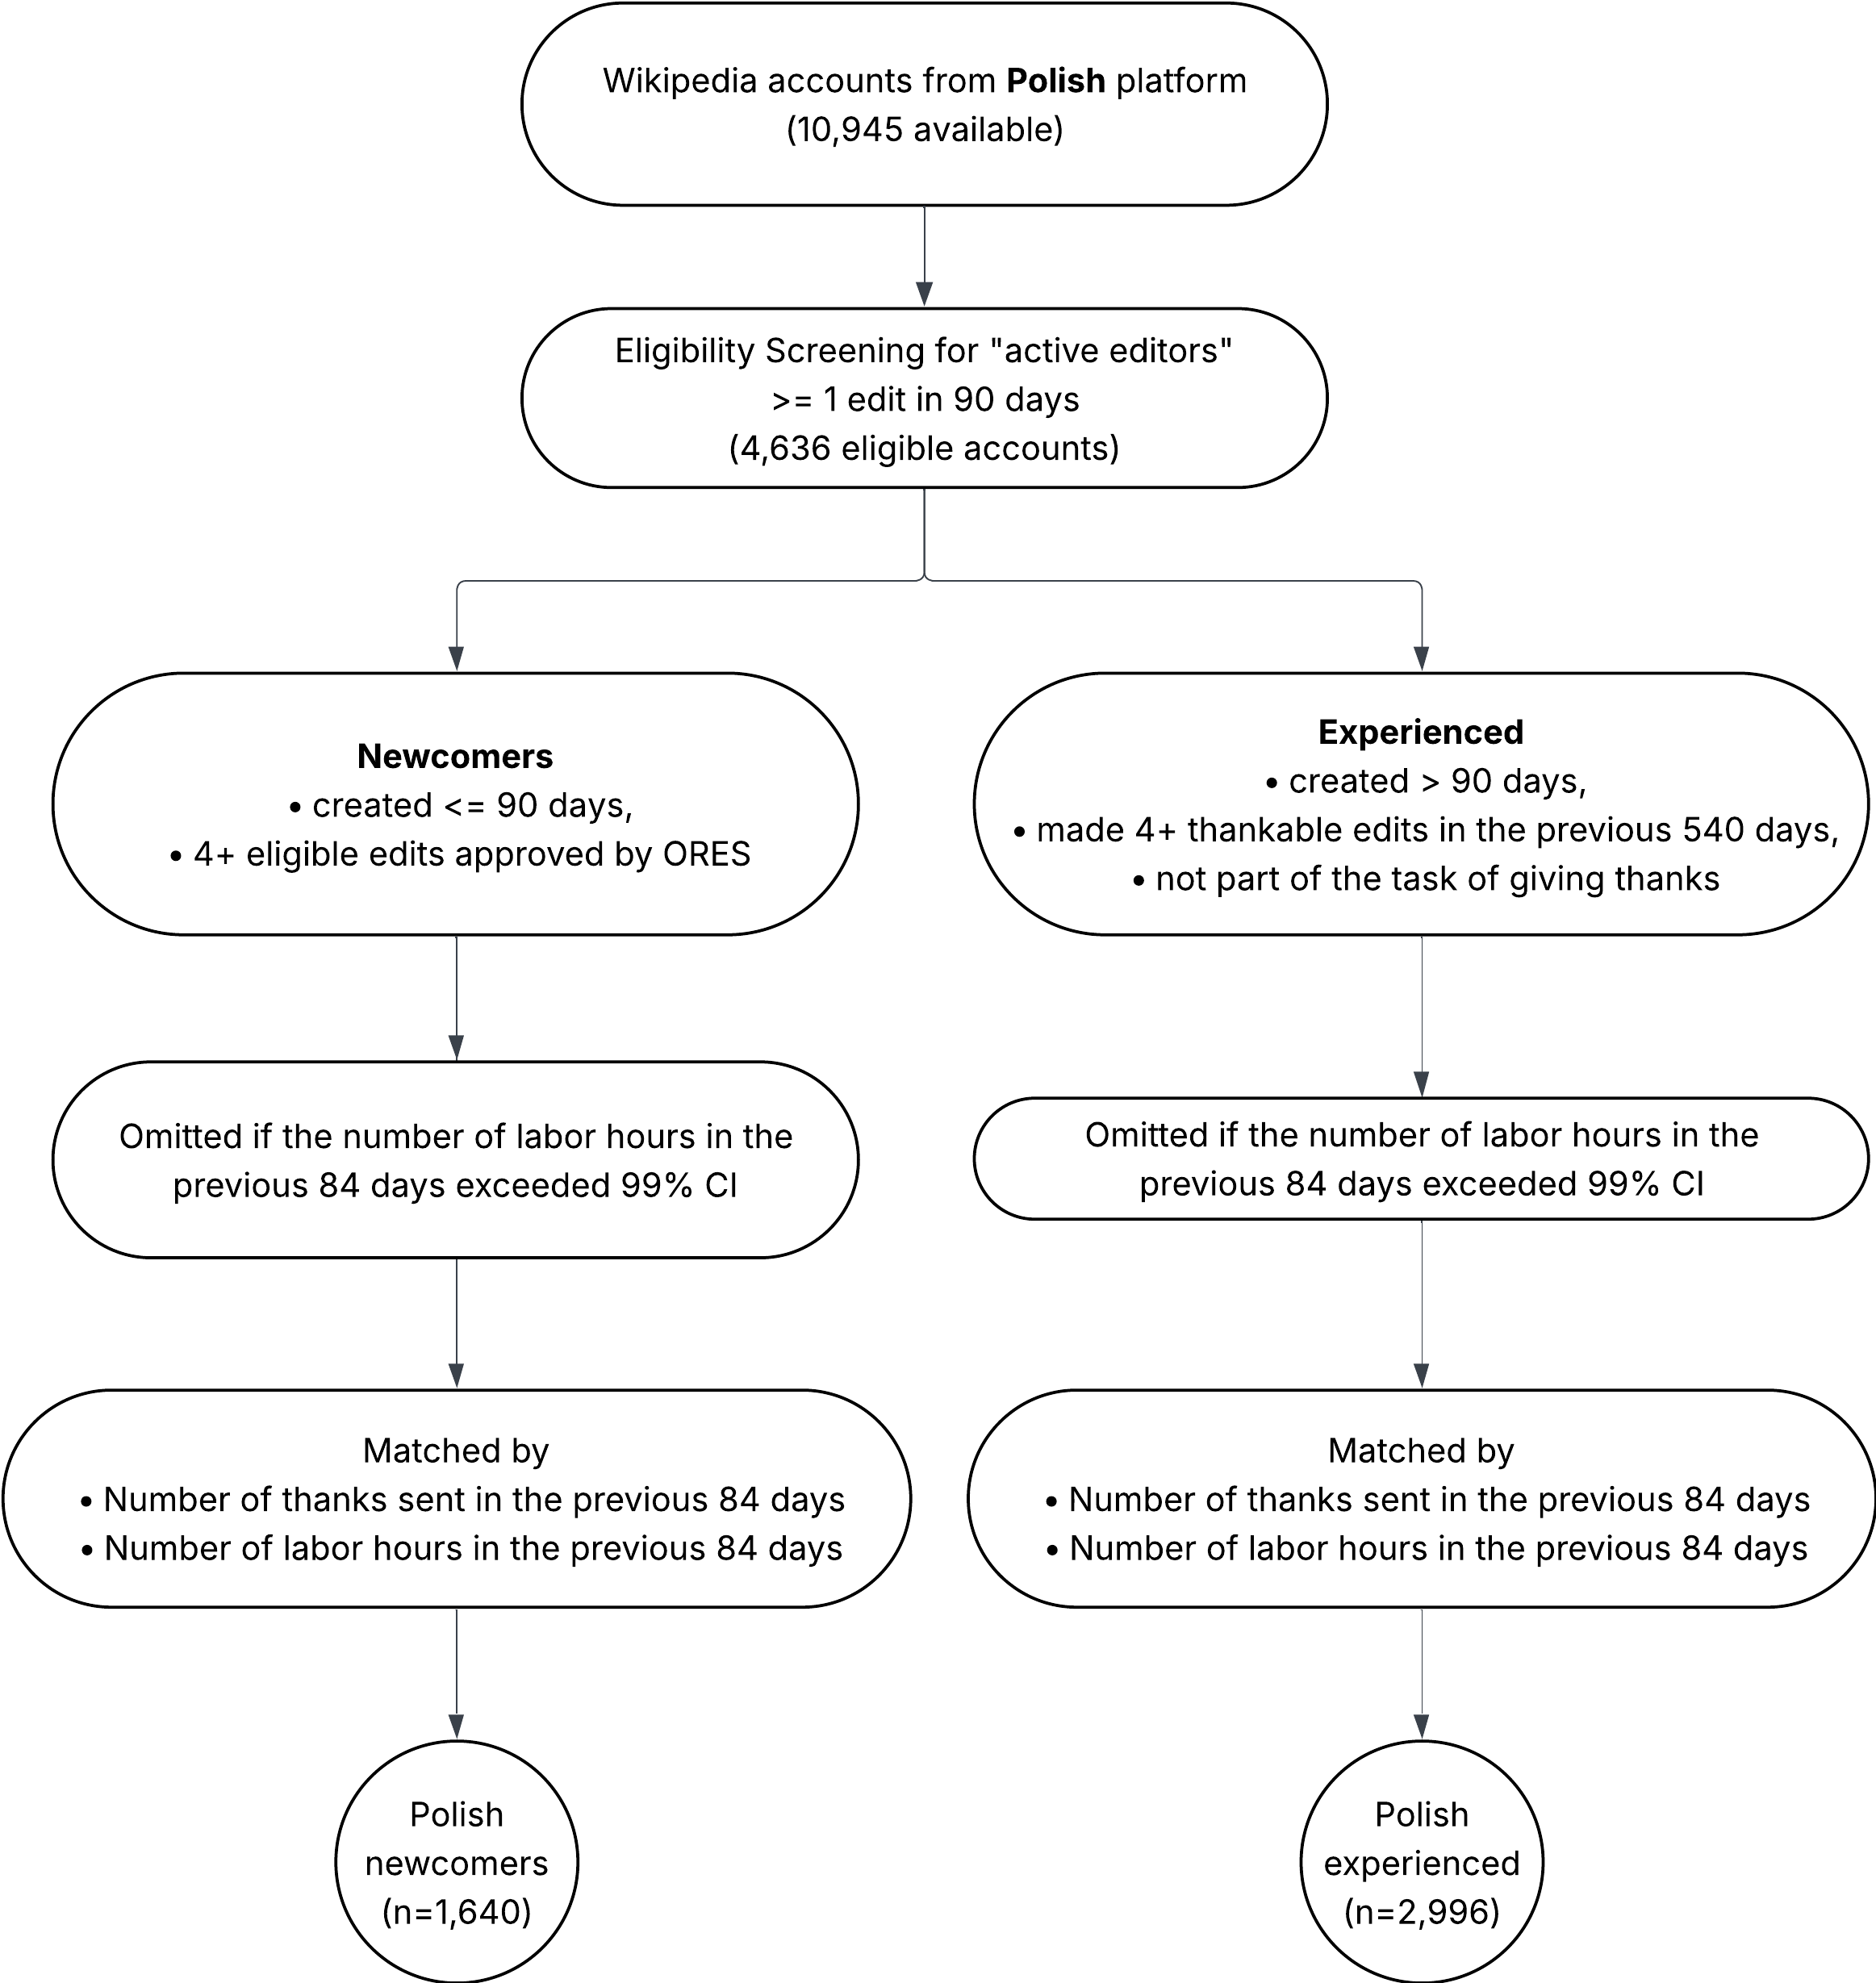
\includegraphics[width=0.85\linewidth]{figs/flow_eligibility_pl.png}
    \caption{\textbf{(a)}~Per-language eligibility and matched-pair construction pipeline, illustrated for Polish Wikipedia. Starting from 10{,}945 available Polish accounts, an activity screen ($\geq$1 edit in the previous 90 days) yielded 4{,}636 active editors, partitioned into \textbf{newcomers} (account $\leq$90 days old; $\geq$4 ORES-approved good-faith edits) and \textbf{experienced contributors} (account $>$90 days old; $\geq$4 thankable edits in the previous 540 days; not engaged in giving thanks for this study). Accounts whose previous-84-day labor hours exceeded the upper 99\% CI were dropped as outliers; remaining accounts were grouped into matched pairs on prior thanks sent and previous-84-day labor hours, yielding 1{,}640 newcomers and 2{,}996 experienced contributors entering the experiment in Polish. The same independent per-language pipeline was applied in Arabic, German, and Persian Wikipedia (see \emph{Cross-Language Implementation}); the four parallel pipelines together produce the 15{,}558 randomized accounts shown in the top row of panel~(b), which presents the pooled CONSORT-style flow from randomization through outcome measurement.}
    \label{fig:eligibility-pl}
\end{figure}

\clearpage
\begin{figure}[p]
    \ContinuedFloat
    \centering
    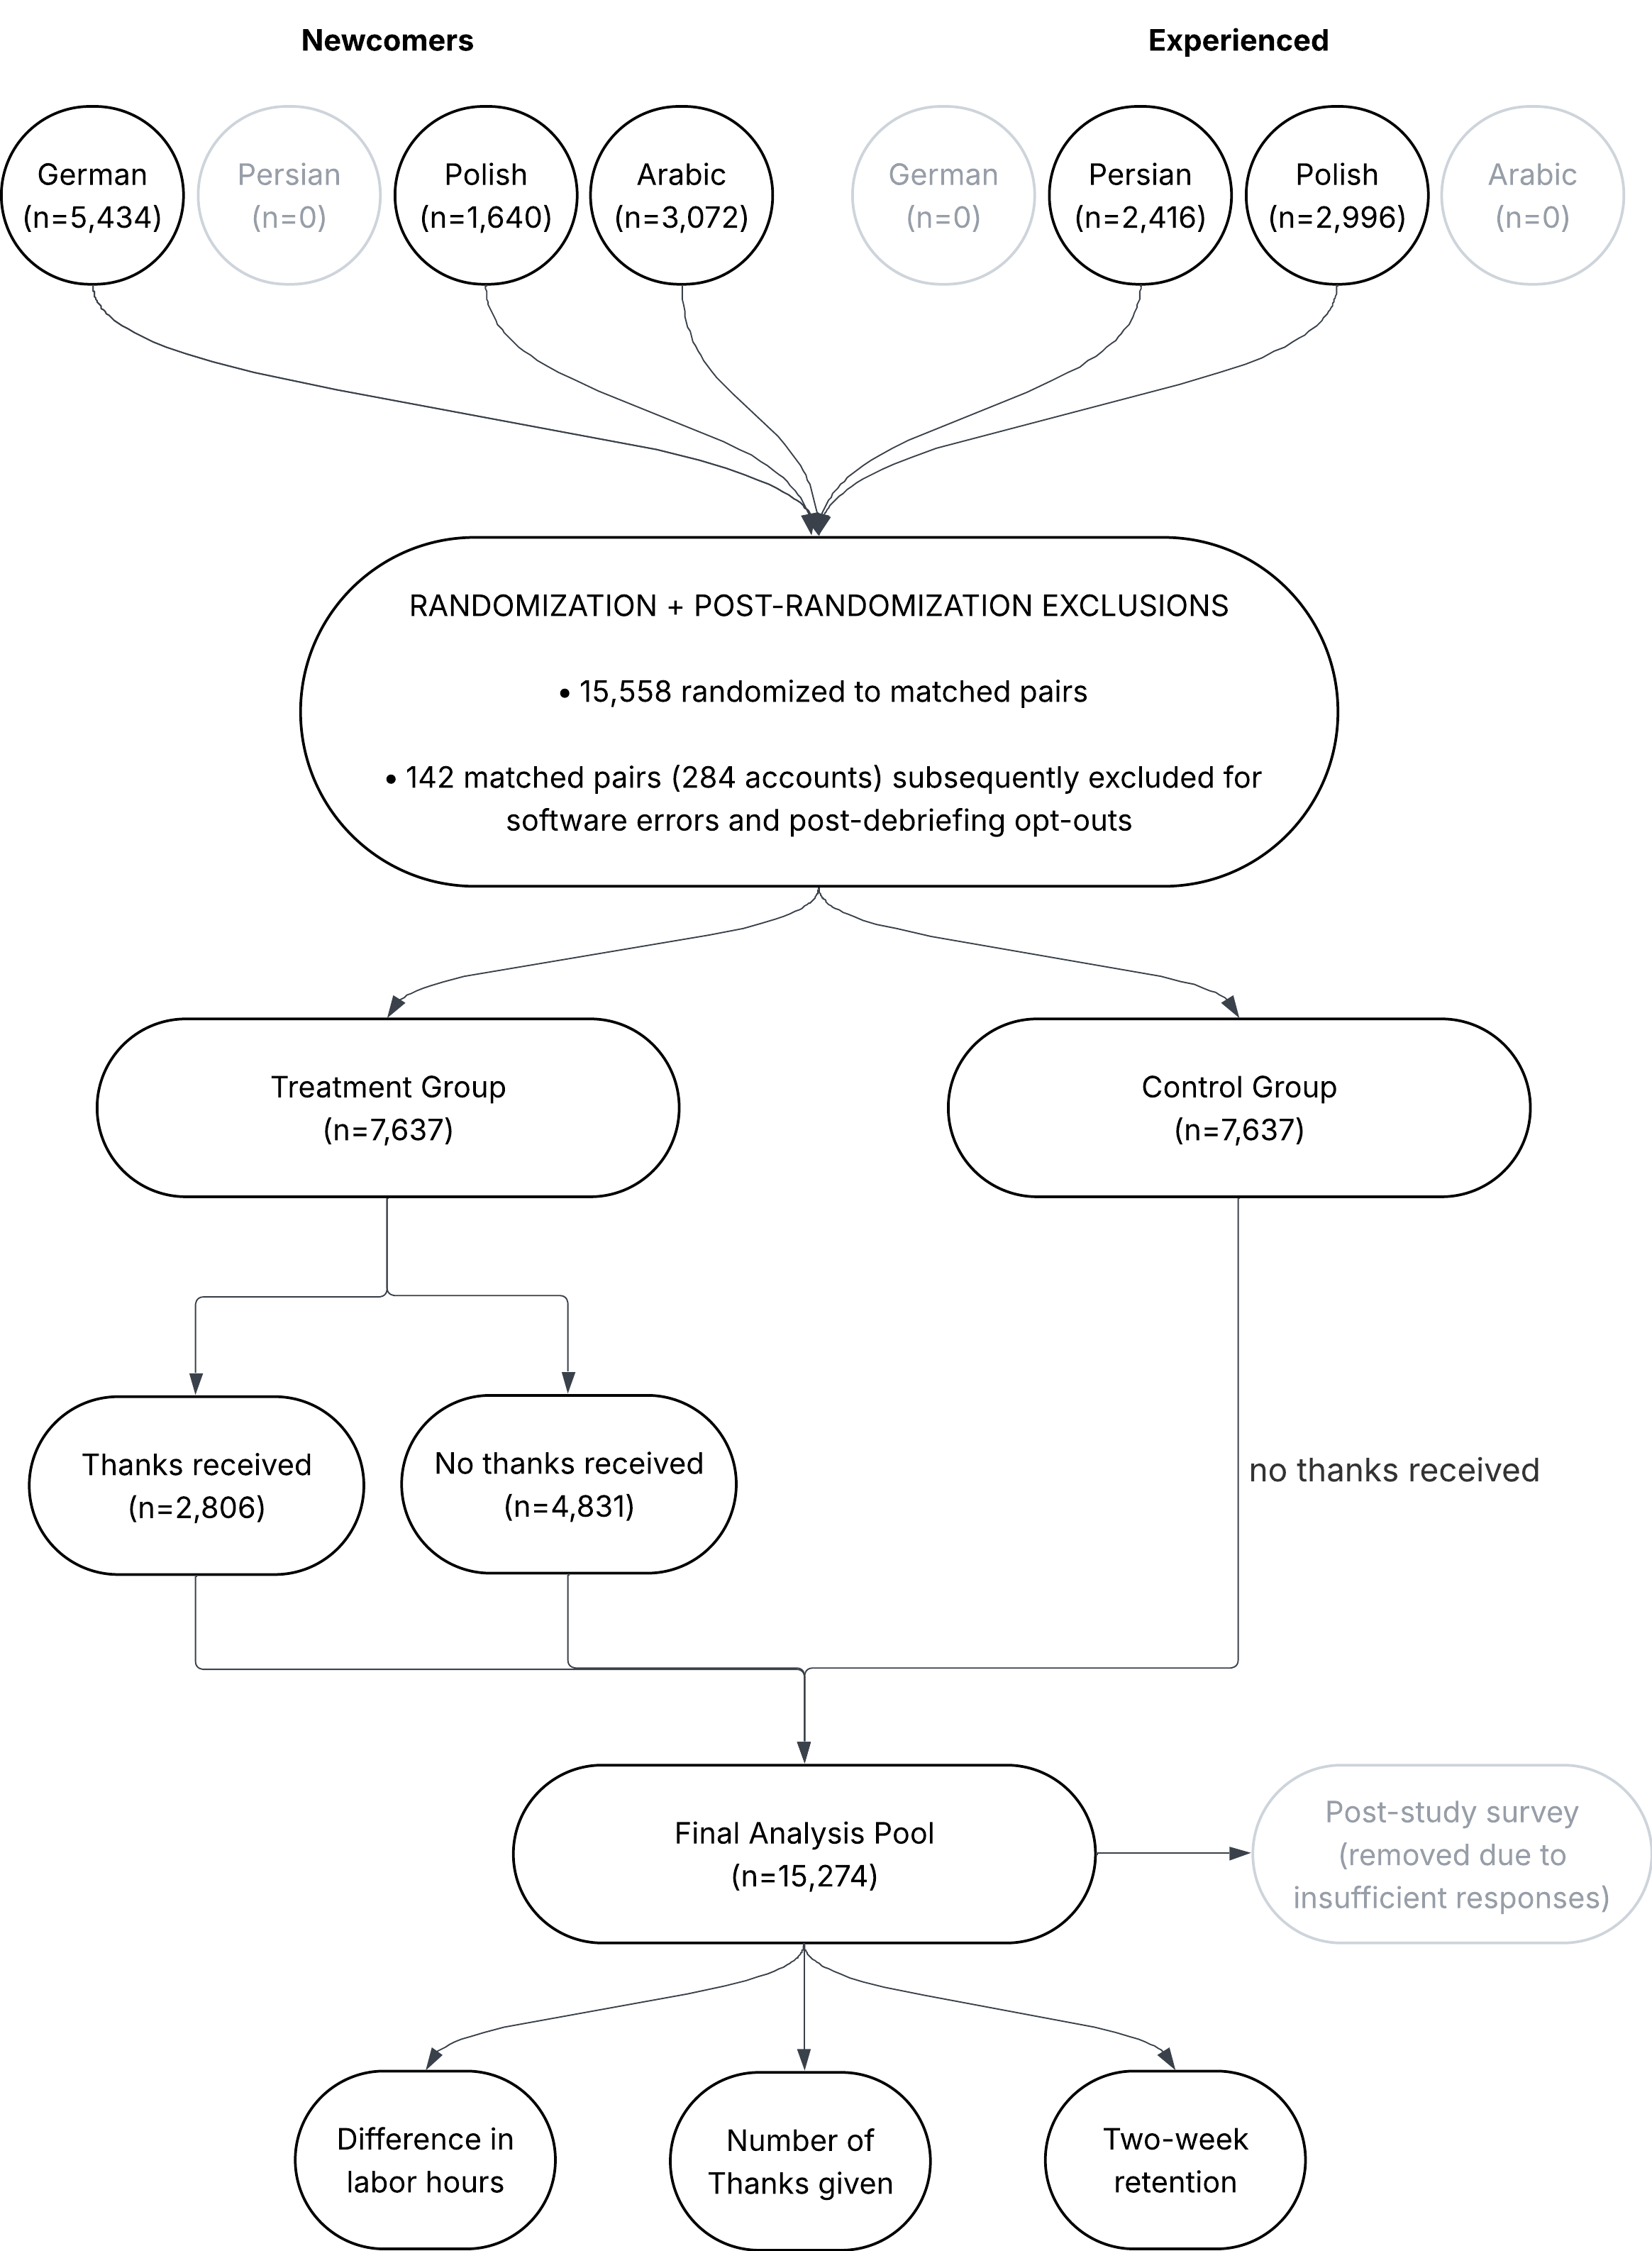
\includegraphics[width=0.9\linewidth]{figs/flow_consort.png}
    \caption{\textbf{(b)}~Pooled CONSORT-style flow diagram beginning at the matched-pair randomization step. The top row shows the eligible matched population by language and experience subgroup, where the outputs of the per-language pipelines are in panel~(a), matching the main-text Table~1 (cells with $n=0$ were excluded a priori for the reasons set out in \emph{Cross-Language Implementation}). Of the 15{,}558 randomized accounts, 142 matched pairs (284 accounts) were subsequently excluded for software errors and post-debriefing opt-outs (Table~\ref{table:predrop_results}); the allocation, treatment-delivery, and final-pool counts shown reflect the resulting $n=15{,}274$ analysis pool used throughout the main text. The grayed \emph{Post-study survey} block was a planned secondary outcome not analysed due to insufficient response rates.}
    \label{fig:consort}
\end{figure}


\clearpage
\begin{table}
\centering
\caption{Pre-registered intent-to-treat (ITT) estimates of average treatment effects (ATE) among Wikipedia participants. Columns: \textit{Estimator} = statistical model used (NegBin = negative binomial regression; DiM = difference in means; Tweedie = Tweedie generalized linear mixed model); \textit{Group} = participant subgroup analyzed (``All'' = all 15,274 participants; ``Newcomers'' = accounts $<$90~days old at enrollment); \textit{N} = sample size; \textit{ATE} = estimated average treatment effect (NegBin: additional thanks sent; DiM: difference in proportions or means; Tweedie: log-scale coefficient); \textit{SE} = standard error. P-values adjusted for multiple comparisons (Holm method) except for manipulation check. The pre-registered analysis specified DiM on the post-minus-pre labor-hours-per-day difference; we report both the original DiM estimate (row marked $\dagger$) and the Tweedie estimate that replaced it after diagnostic comparison (see \textit{Reliably Estimating the Effect on Labor Hours}).}
\label{table:preregresults}
\begin{tabular}{l c c c c c c}
\hline
Outcome & Estimator & Group & N & ATE & SE & \textit{p} \\
\hline
Thanks sent & NegBin & All &
  $15,274$ &
  $0.47$ &
  $0.14$ &
  $0.0021$ \\
Two-week retention & DiM & All &
  $15,274$ &
  $0.022$ &
  $0.006$ &
  $0.00093$ \\
Labor hours per day & Tweedie & Newcomers &
  $9,984$ &
  $0.43$ &
  $0.08$ &
  $<$0.0001 \\
Labor hours/day diff.\ $^{\dagger}$ & DiM & Newcomers &
  $9,984$ &
  $0.003$ &
  $0.002$ &
  $0.13$ \\
Manipulation check & DiM & All &
  $767$ &
  $0.29$ &
  $0.035$ & $<$0.0001 \\
\hline
\end{tabular}
\end{table}




\clearpage
\begin{table}[ht]
\centering
\small
\caption{First-generation thanks delivered to study participants by Wikipedia language community. The study ran six waves between August 2, 2019 and February 11, 2020, during which a total of 313 volunteer thankers were recruited across all four communities. Per-community thanker counts and per-thanker distributions of thanks sent are not reported because the Superthanker application did not retain a complete sender-identified log of first-generation thanks.}
\label{table:thankers}
\begin{tabular}{l r}
\toprule
\textbf{Language} & \textbf{First-gen thanks sent} \\
\midrule
Arabic  & 199 \\
German  & 1{,}319 \\
Persian & 88 \\
Polish  & 1{,}200 \\
\midrule
\textbf{Total} & \textbf{2{,}806} \\
\bottomrule
\end{tabular}
\end{table}


\clearpage
\begin{table}
\centering
\caption{Performance of machine learning models used to flag good-faith edits for volunteer review, drawn from Wikimedia Foundation model documentation for Arabic (\url{https://meta.wikimedia.org/wiki/Machine_learning_models/Production/Arabic_Wikipedia_goodfaith_edit}), Persian (\url{https://meta.wikimedia.org/wiki/Machine_learning_models/Production/Persian_Wikipedia_goodfaith_edit}), and Polish (\url{https://meta.wikimedia.org/wiki/Machine_learning_models/Production/Polish_Wikipedia_goodfaith_edit}). \textit{Precision} = fraction of flagged edits that were genuinely good-faith (relevant to volunteers, who should only see high-quality edits to thank); \textit{Recall} = fraction of all genuine good-faith edits that were flagged (relevant to coverage of eligible contributors). German Wikipedia was excluded because machine learning was not used for participant selection in that community.}
\label{table:mlresults}
\begin{tabular}{l c c c c}
\textbf{Language} & \textbf{Model} &  \textbf{Test Data N} & \textbf{Precision} & \textbf{Recall} \\
\hline
\href{https://meta.wikimedia.org/wiki/Machine_learning_models/Production/Arabic_Wikipedia_goodfaith_edit}{Arabic} & Good Faith & 18,208 & 0.994 & 0.999 \\
\href{https://meta.wikimedia.org/wiki/Machine_learning_models/Production/Persian_Wikipedia_goodfaith_edit}{Persian} & Good Faith & 18,150 & 0.989 & 0.997 \\
\href{https://meta.wikimedia.org/wiki/Machine_learning_models/Production/Polish_Wikipedia_goodfaith_edit}{Polish} & Good Faith & 4,772 & 0.987 & 0.998 \\
\end{tabular}
\end{table}

\clearpage
\begin{figure}[p]
    \centering
    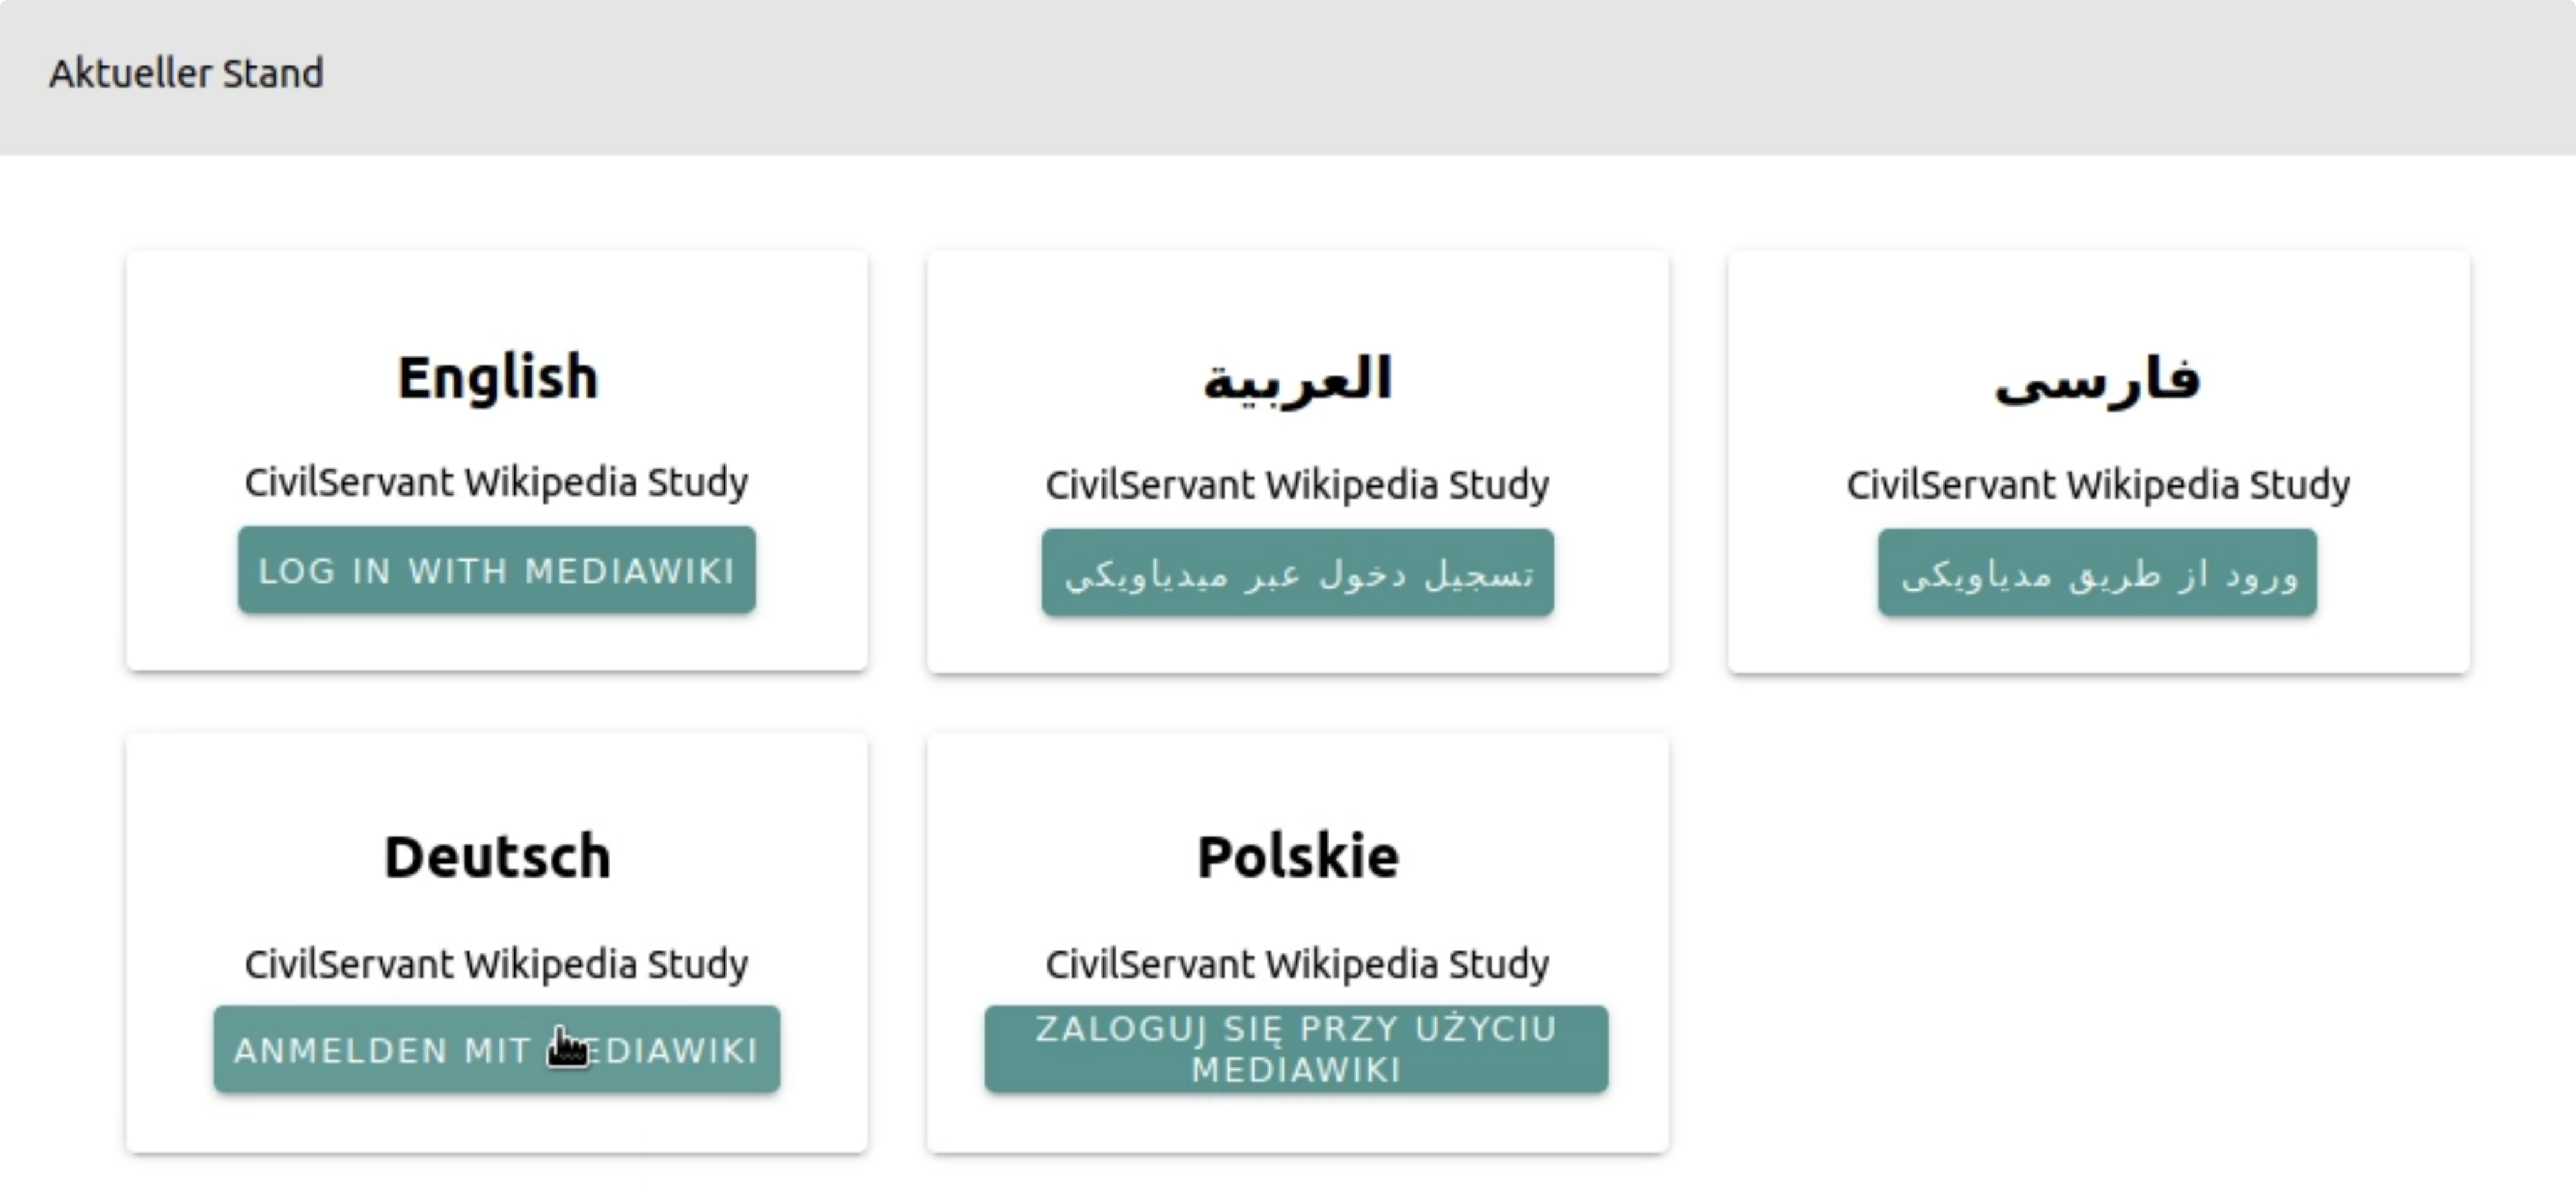
\includegraphics[width=0.85\linewidth]{figs/ui_01_landing.png}
    \caption{\textbf{(a)}~Language-selection landing page of the Superthanker volunteer software interface. The screenshot illustrates the German community version of the interface; right-hand callouts label each on-screen element in English (this convention is followed throughout panels~(a)--(f), so the prose below uses English labels). Volunteers chose their Wikipedia community (Arabic, Persian, German, Polish, or English) and clicked \emph{Log in with MediaWiki}. The cards of different language communities were the workflow entry points for trained volunteer-thankers.}
    \label{fig:ui-walkthrough}
\end{figure}

\clearpage
\begin{figure}[p]
    \ContinuedFloat
    \centering
    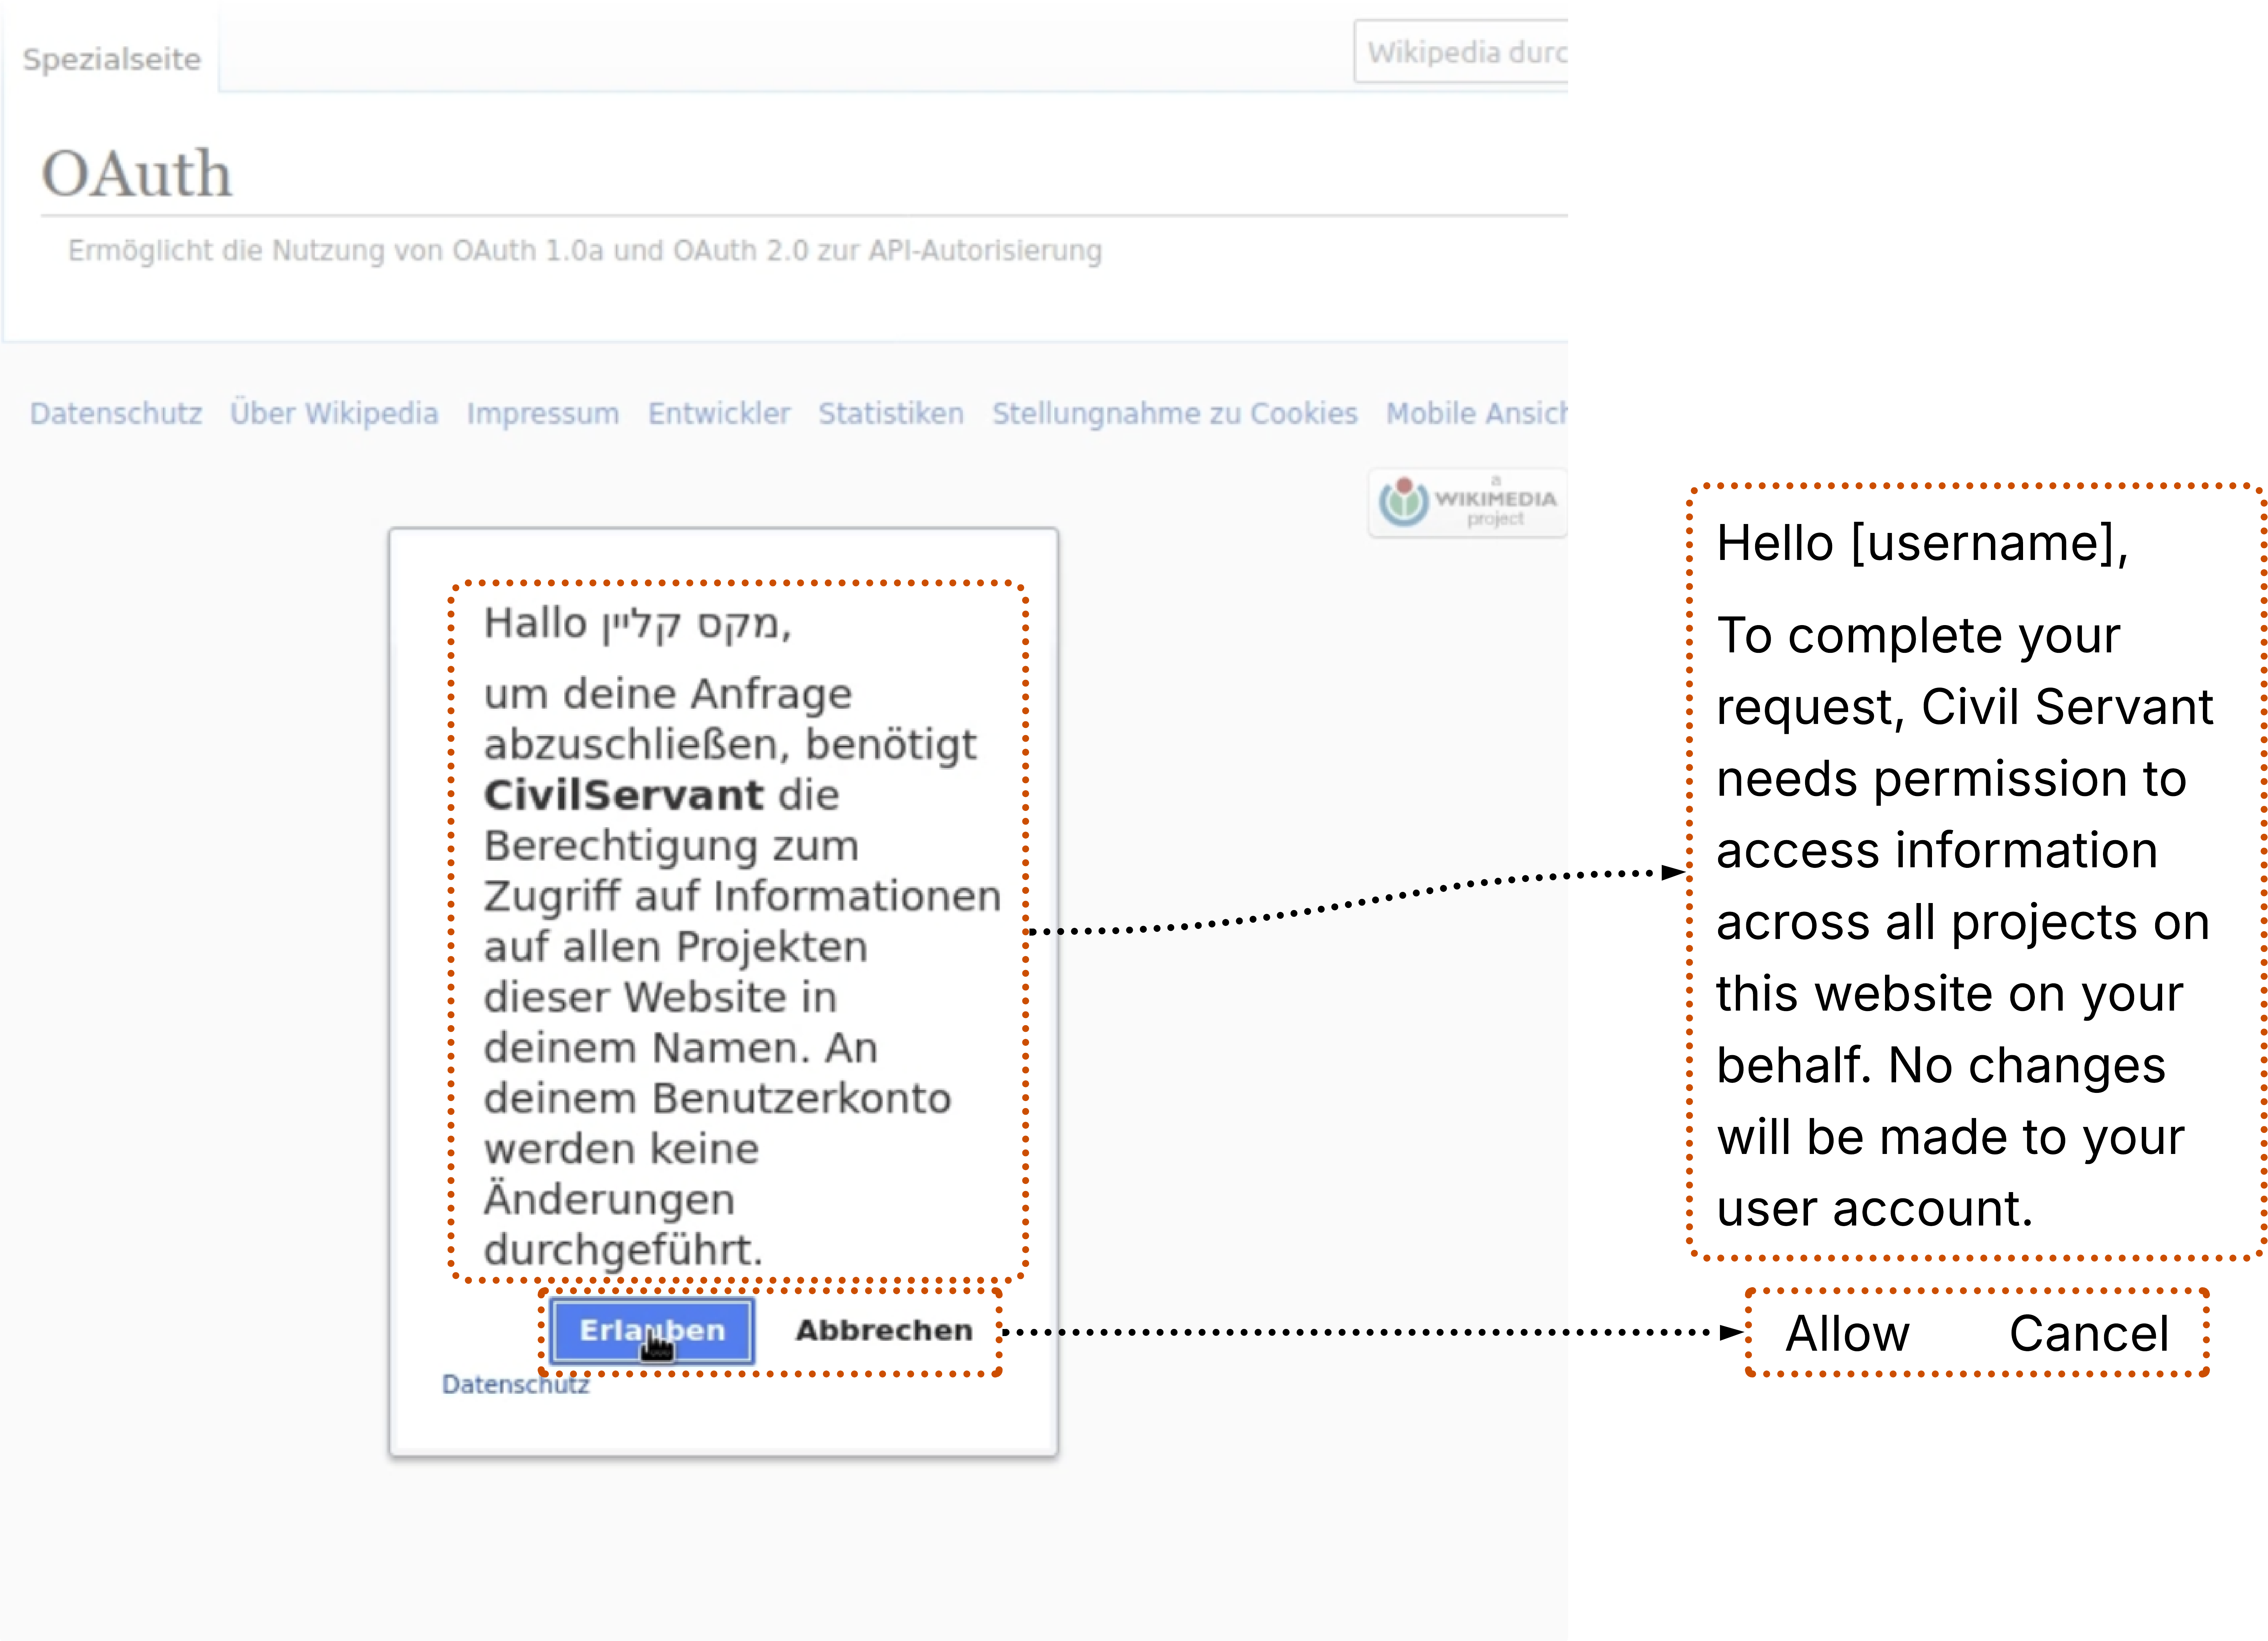
\includegraphics[width=0.95\linewidth]{figs/ui_02_oauth.png}
    \caption{\textbf{(b)}~OAuth authorisation step. Wikipedia's standard OAuth flow asked the volunteer to grant the Civil Servant application read-only permission to access information about their account across Wikimedia projects, with no permission to make changes on the volunteer's behalf. Clicking \emph{Allow} advanced the volunteer to the welcome screen; \emph{Cancel} returned them to the landing page.}
\end{figure}

\clearpage
\begin{figure}[p]
    \ContinuedFloat
    \centering
    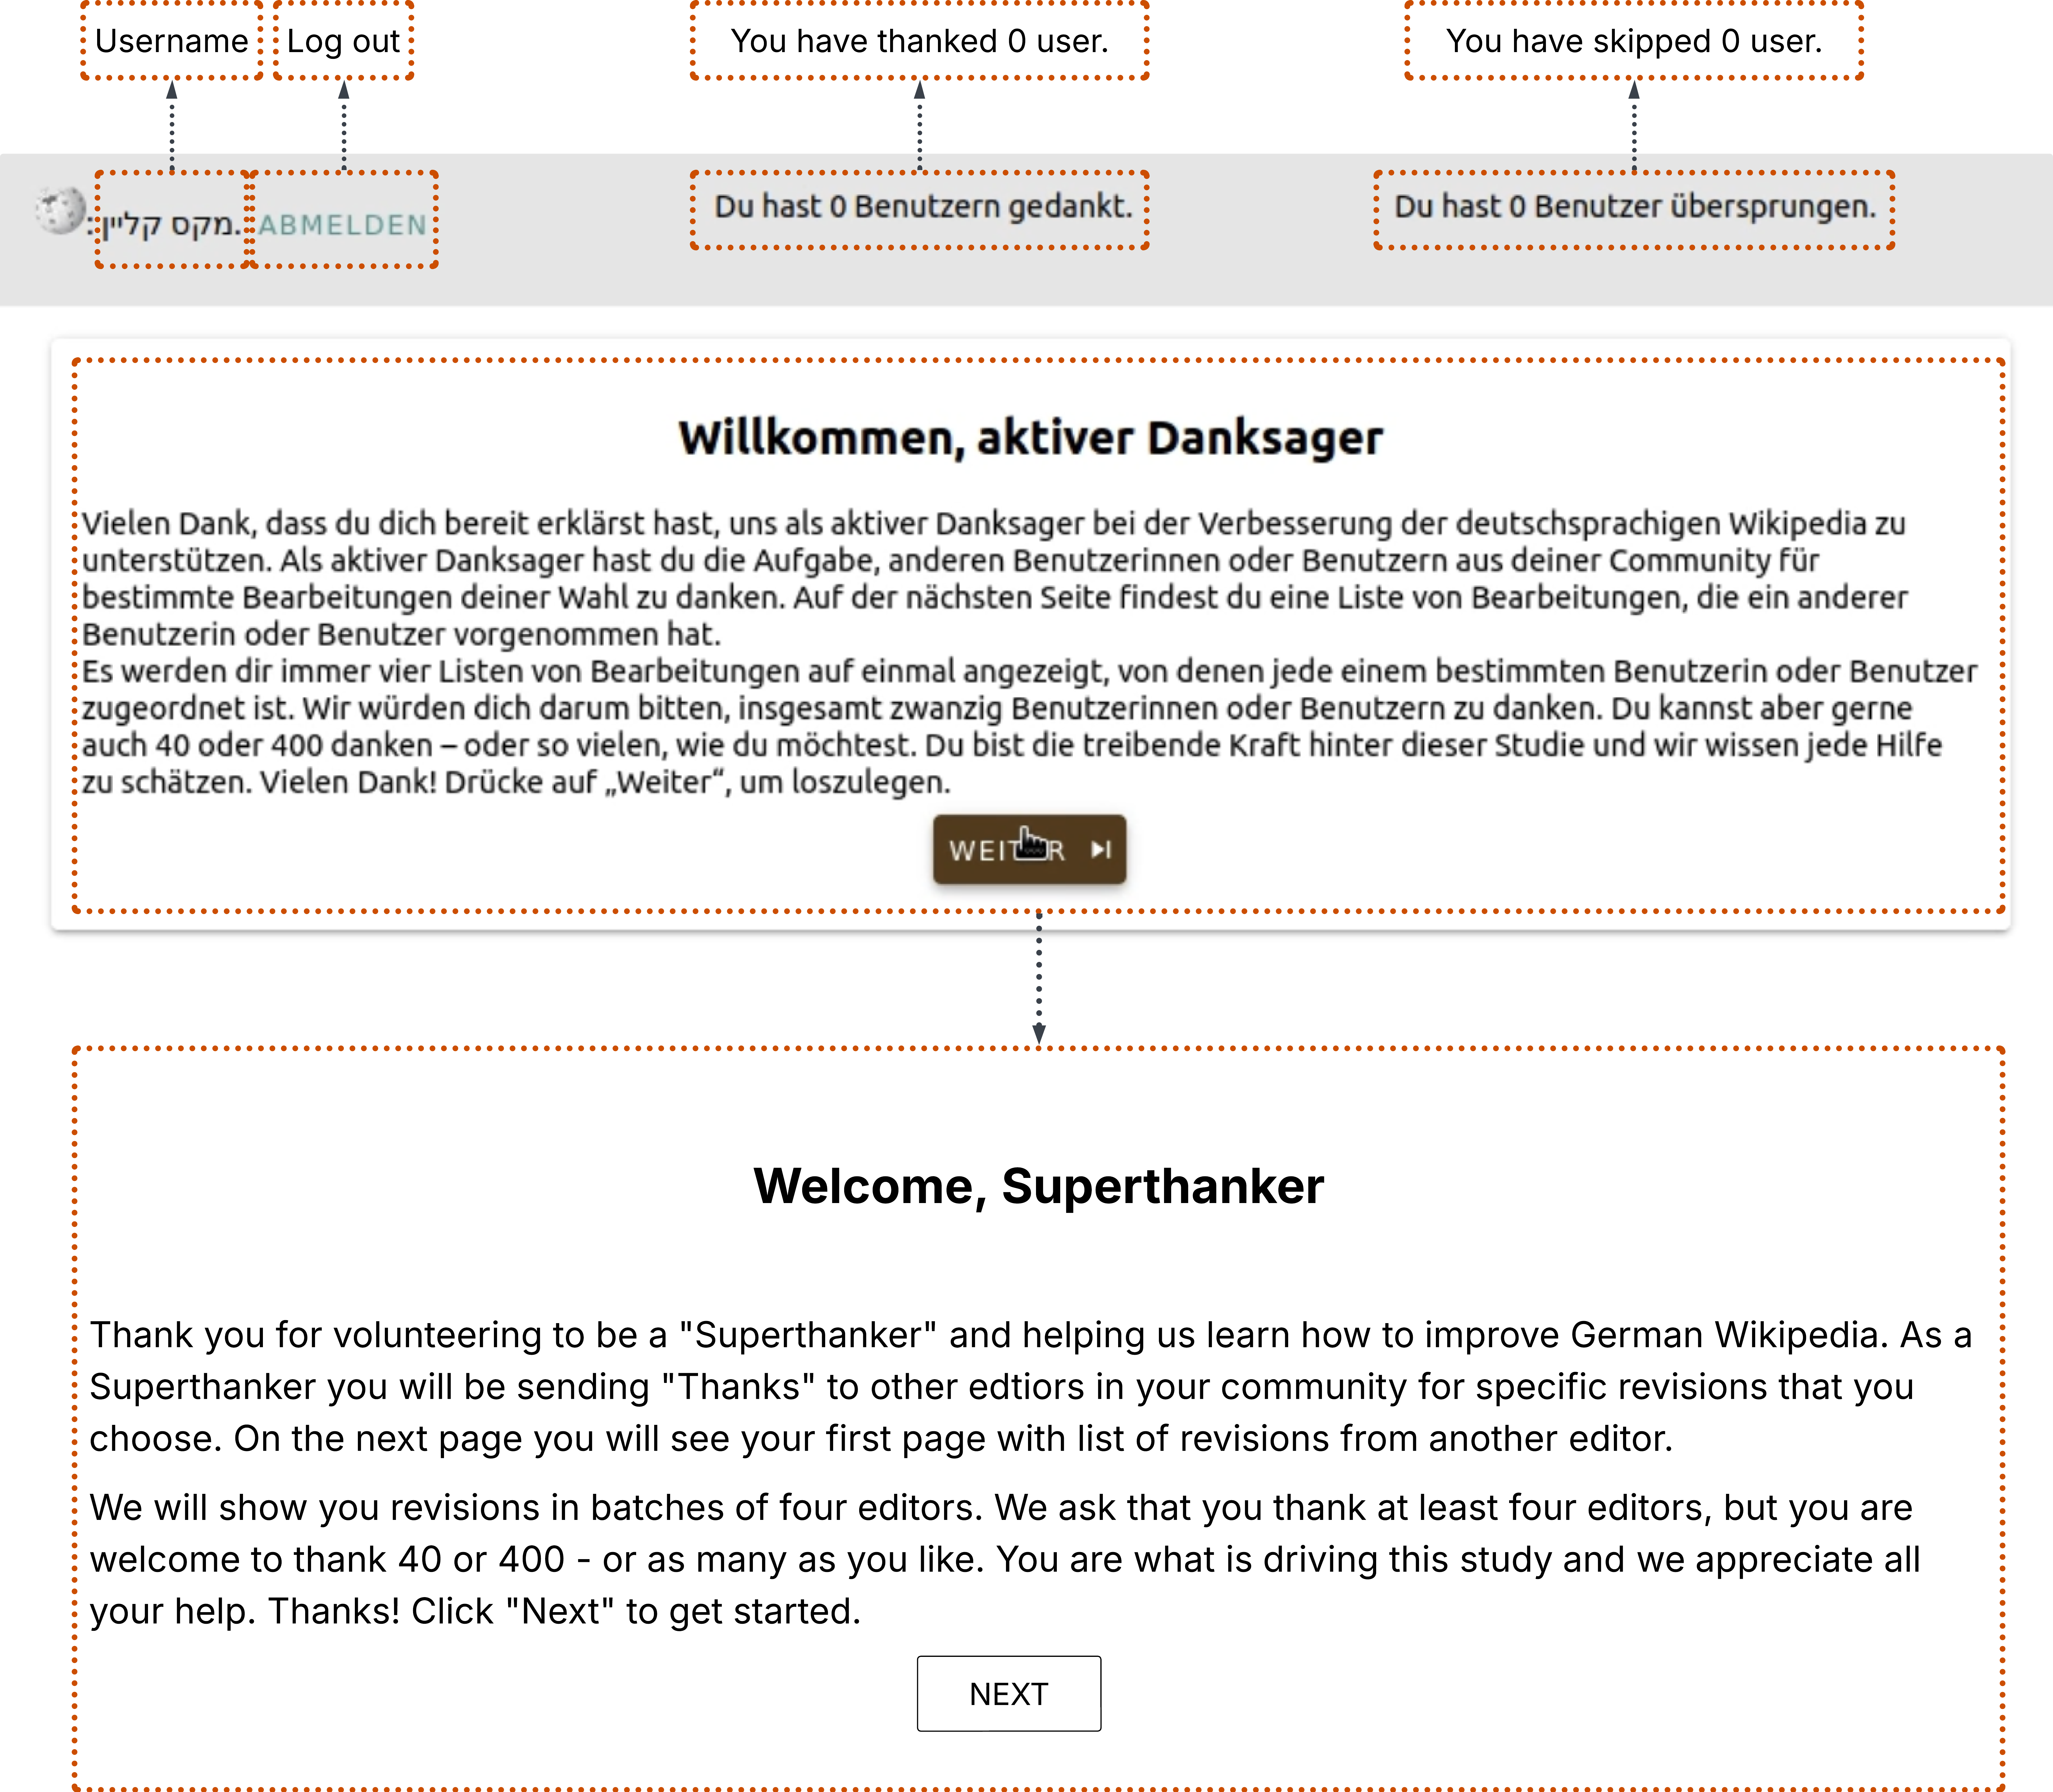
\includegraphics[width=0.85\linewidth]{figs/ui_03_welcome.png}
    \caption{\textbf{(c)}~Welcome screen displayed after authentication. The persistent header at the top of every page shows the volunteer's username, a \emph{Log out} button, and live counters reporting thanks sent and skipped during the current session. The body text welcomes the volunteer and describes the task: volunteers were asked to thank at least four editors in total by selecting one revision from each batch of four candidate editors and clicking \emph{Thank}. Clicking \emph{Next} opened the first batch of candidate revisions.}
\end{figure}

\clearpage
\begin{figure}[p]
    \ContinuedFloat
    \centering
    \includegraphics[width=0.7\linewidth]{figs/ui_04_thanking.png}
    \caption{\textbf{(d)}~Annotated detail view of the main thanking interface. For each volunteer thanker, the application presented two side-by-side revision options (\emph{Edit Option~\#1} and \emph{\#2}). Right-hand boxes labeled each interface element: (1)~task instructions; (2)~the \emph{Edit Option} header; (3)~the article title (linked to Wikipedia); (4)~timestamp, edit-code link, and editor ID for the original edit; (5)~timestamp, edit-code link, and editor ID for the new edit; (6)~the line number; (7)~context before the revised area; (8)~the previous version of the revised text (left column of the diff); (9)~the new version of the revised text (right column), highlighted using Wikipedia's standard diff conventions; (10)~context after the revised area; (11)~the \emph{Thank} button; and (12)~the \emph{Skip these users} button. See \url{https://en.wikipedia.org/wiki/Help:Diff} for more on Wikipedia's diff conventions.}
\end{figure}

\clearpage
\begin{figure}[p]
    \ContinuedFloat
    \centering
    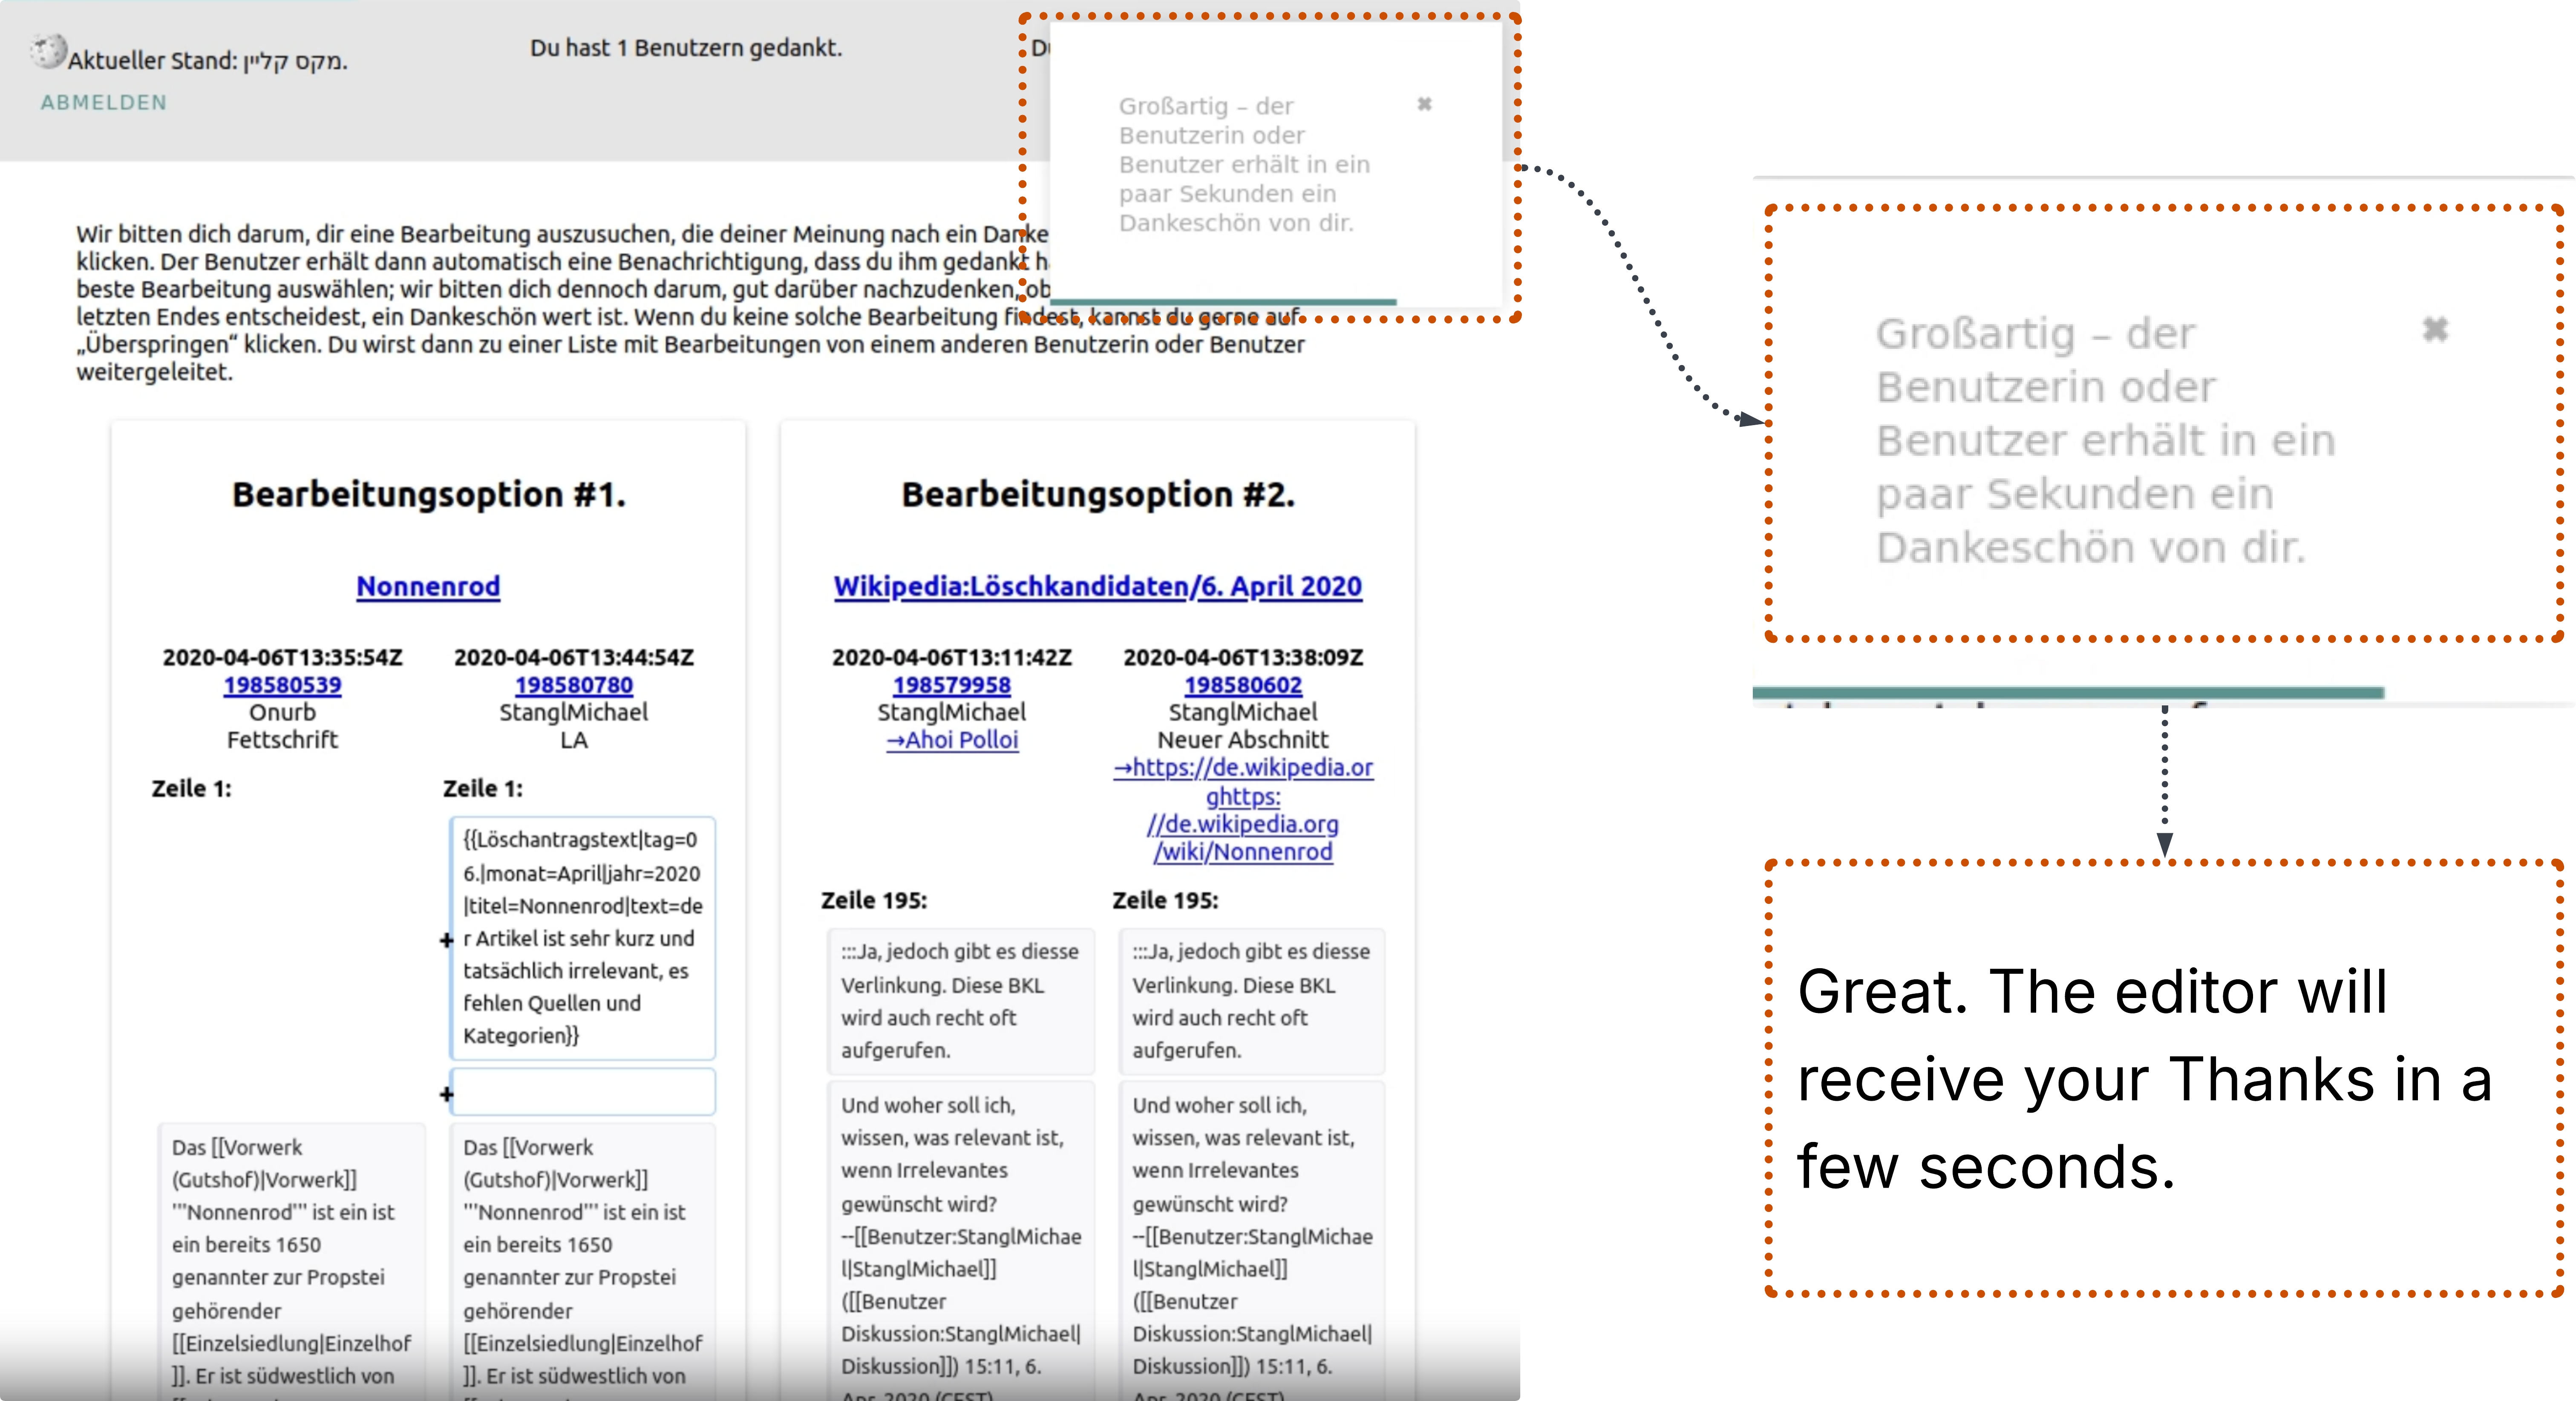
\includegraphics[width=0.95\linewidth]{figs/ui_05_confirmation.png}
    \caption{\textbf{(e)}~Post-thank confirmation. Immediately after the volunteer clicked \emph{Thank}, a notification at the top of the page (with English translation in the right-hand callout) reported \emph{Great. The editor will receive your Thanks in a few seconds}, and the persistent header counter incremented to \emph{You have thanked 1 user}.}
\end{figure}

\clearpage
\begin{figure}[p]
    \ContinuedFloat
    \centering
    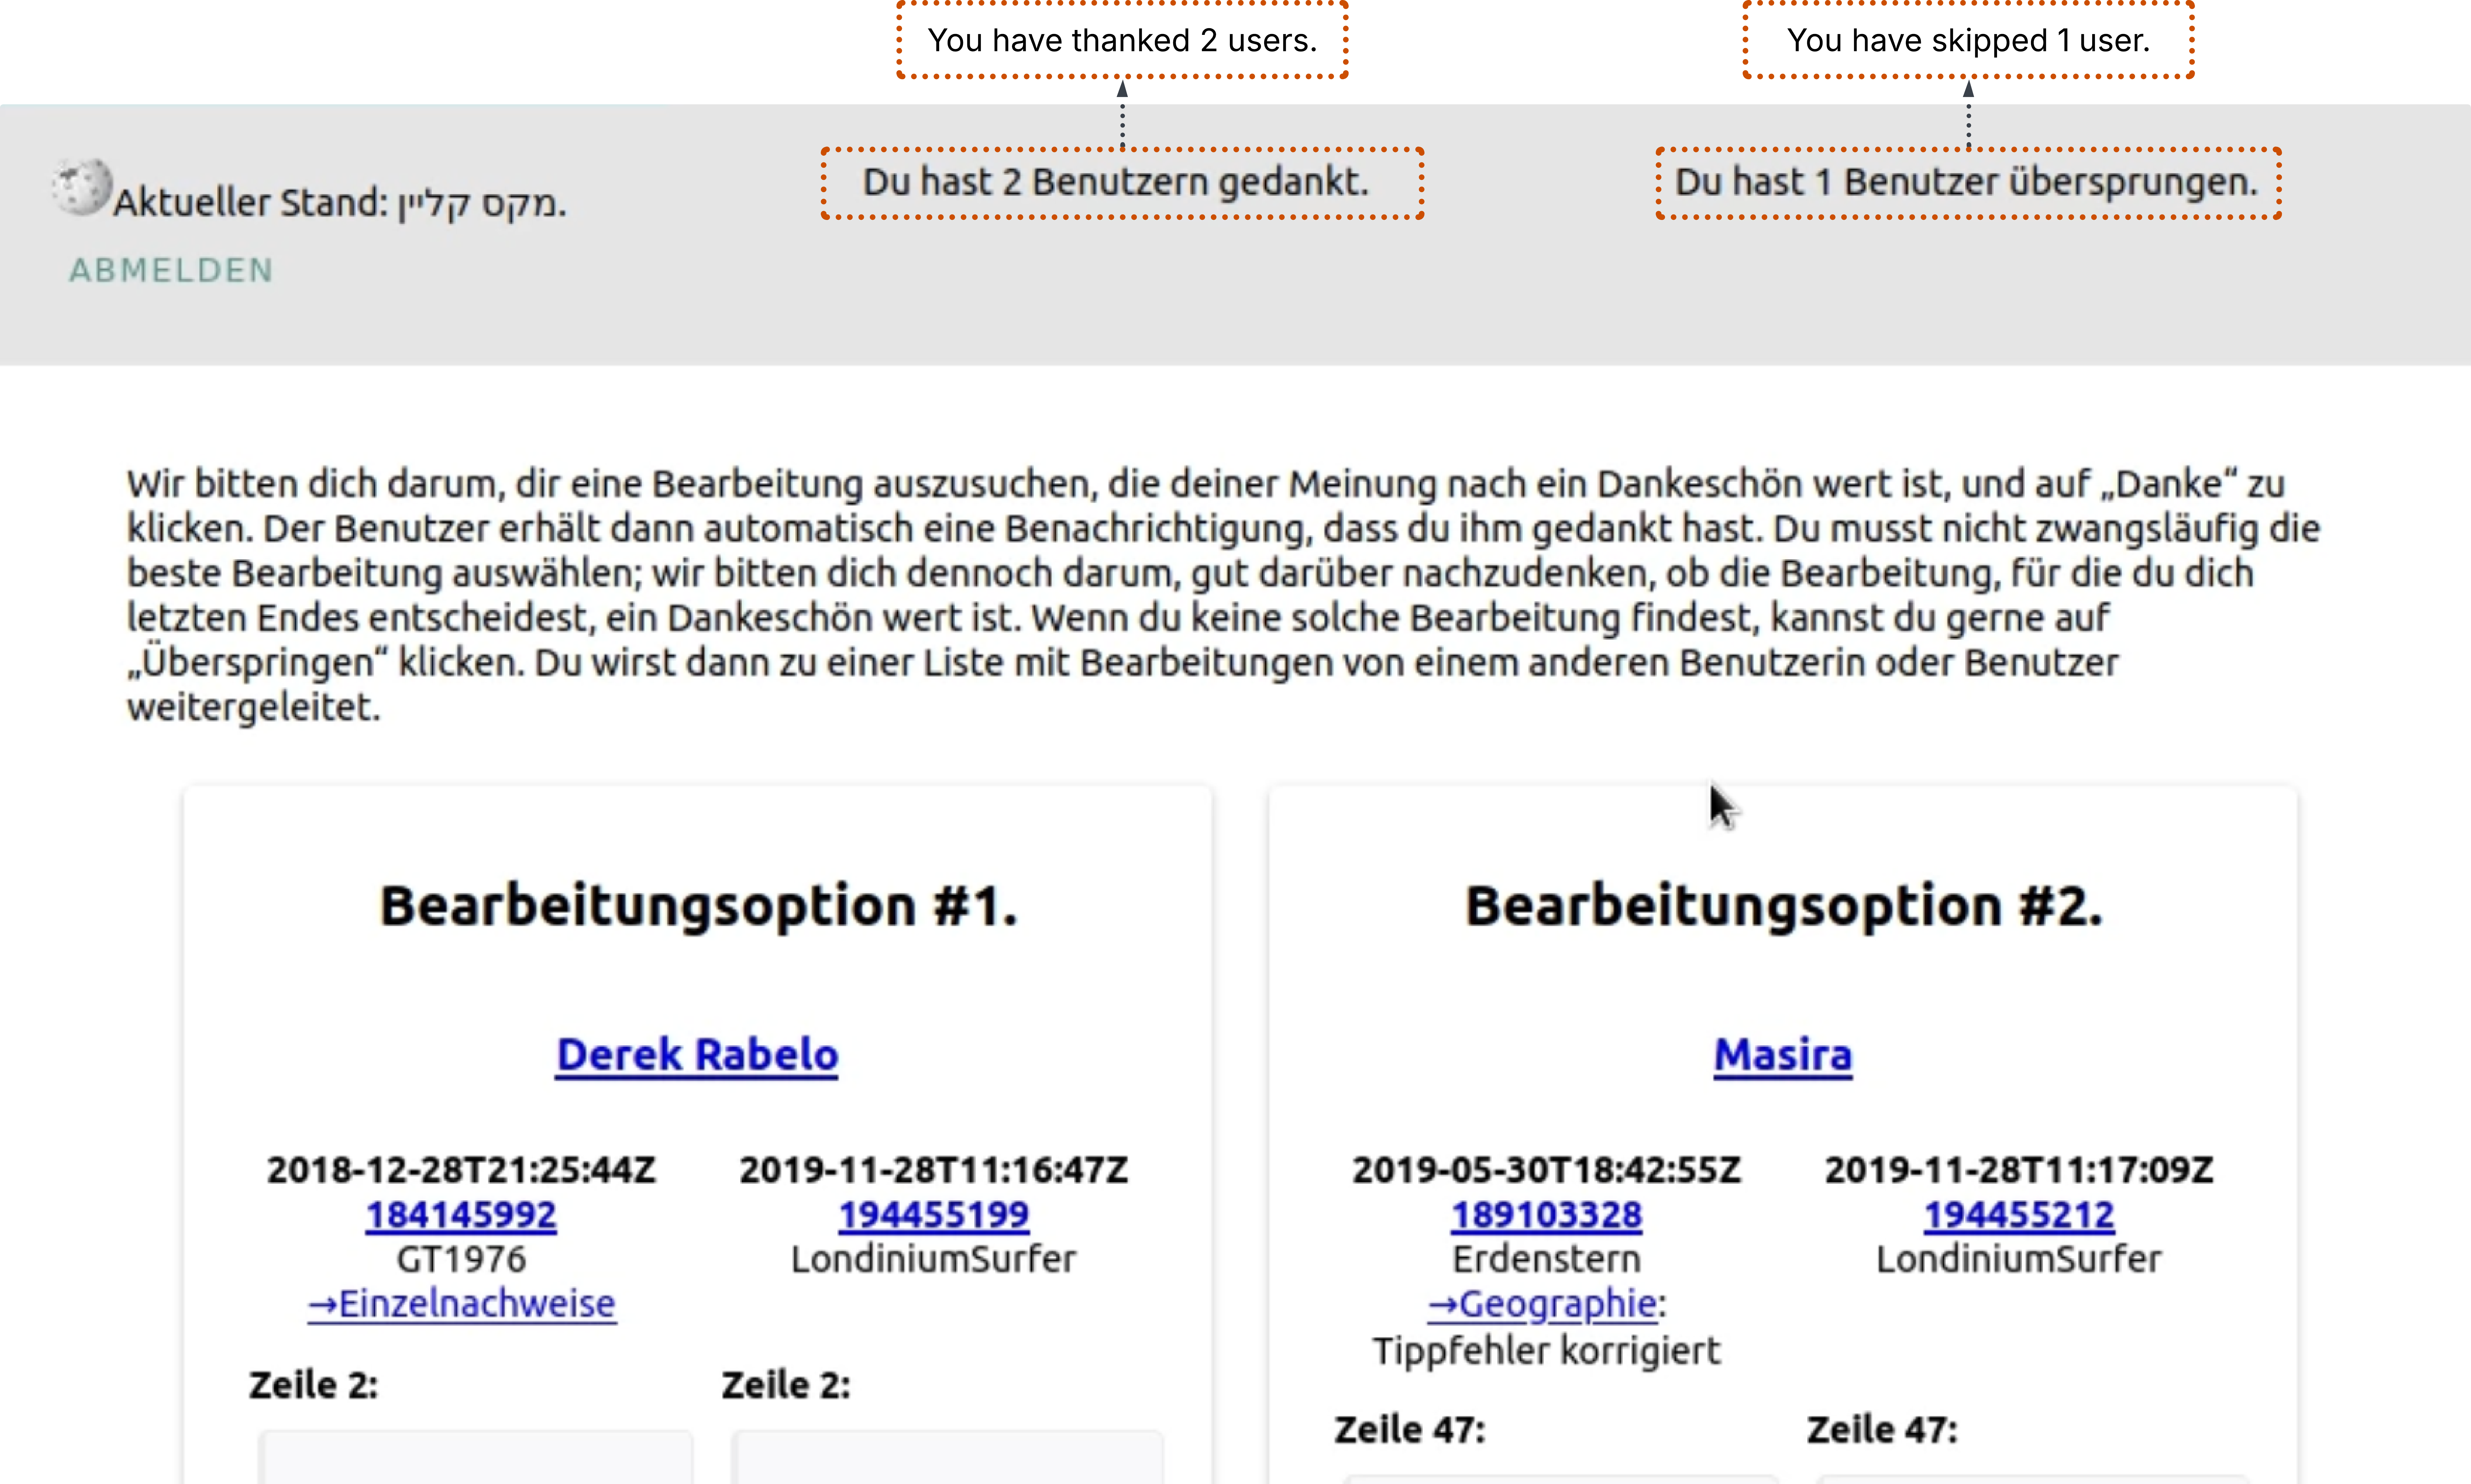
\includegraphics[width=0.95\linewidth]{figs/ui_06_counters.png}
    \caption{\textbf{(f)}~Session-progress counters after multiple thanks. Counters \emph{You have thanked 2 users} and \emph{You have skipped 1 user} updated in real time, giving feedback on session progress.}
\end{figure}


\clearpage
\begin{table*}[t]
\centering
\caption{Balance table comparing pre-treatment characteristics of treatment and control groups. P-values are from Wilcoxon rank-sum tests (continuous variables) or chi-squared tests (categorical variables). Std.~Diff.~is Cohen's $d$ for continuous and binary variables or Cram\'er's $V$ for multi-category variables. With $N > 15{,}000$, small p-values can arise from trivially small differences; all $|d| < 0.05$ for genuine pre-treatment covariates confirm negligible imbalance. The large standardized difference for \textit{Thanks received (pre-study)} ($d = 1.05$) is expected: receiving a first-generation thank is the treatment itself, so by design treated participants have thanks received $> 0$ and control participants have thanks received $= 0$. This row serves as a manipulation check confirming treatment delivery, not a covariate balance diagnostic.}
\label{table:balance}
\begin{tabular}{lrrrll}
\toprule
 & \textbf{Control} & \textbf{Treatment} & \textbf{Total} & \textbf{p-value} & \textbf{Std.~Diff.} \\
 & (N = 7,637) & (N = 7,637) & (N = 15,274) & & \\
\midrule
\multicolumn{6}{l}{\textit{Previous experience category}} \\
\quad Newcomer (0 days) & 4,992 (65.37\%) & 4,992 (65.37\%) & 9,984 (65.37\%) & & \\
\quad 90 days & 255 (3.34\%) & 255 (3.34\%) & 510 (3.34\%) & & \\
\quad 180 days & 280 (3.67\%) & 280 (3.67\%) & 560 (3.67\%) & & \\
\quad 365 days & 429 (5.62\%) & 429 (5.62\%) & 858 (5.62\%) & & \\
\quad 730 days & 476 (6.23\%) & 476 (6.23\%) & 952 (6.23\%) & & \\
\quad 1460 days & 586 (7.67\%) & 586 (7.67\%) & 1,172 (7.67\%) & & \\
\quad 2920 days & 619 (8.11\%) & 619 (8.11\%) & 1,238 (8.11\%) & & \\
\addlinespace
\multicolumn{6}{l}{\textit{Newcomer status}} \\
\quad Newcomer & 4,992 (65.37\%) & 4,992 (65.37\%) & 9,984 (65.37\%) & & \\
\quad Experienced & 2,645 (34.63\%) & 2,645 (34.63\%) & 5,290 (34.63\%) & 1.00 & $<-$0.0001 \\
\addlinespace
\multicolumn{6}{l}{\textit{Language}} \\
\quad Arabic & 1,518 (19.88\%) & 1,518 (19.88\%) & 3,036 (19.88\%) &  &  \\
\quad German & 2,659 (34.82\%) & 2,659 (34.82\%) & 5,318 (34.82\%) &  &  \\
\quad Persian & 1,177 (15.41\%) & 1,177 (15.41\%) & 2,354 (15.41\%) &  &  \\
\quad Polish & 2,283 (29.89\%) & 2,283 (29.89\%) & 4,566 (29.89\%) & 1.00 & 0.00 \\
\addlinespace
\multicolumn{6}{l}{\textit{Pre-study labor hours per day}} \\
\quad Mean (SD) & 0.03 (0.12) & 0.03 (0.11) & 0.03 (0.12) & $<$0.0001 & 0.03 \\
\quad Median & 0 & 0.0034 & 0.0028 & & \\
\addlinespace
\multicolumn{6}{l}{\textit{Pre-study labor hours (total)}} \\
\quad Mean (SD) & 1.24 (4.84) & 1.37 (4.82) & 1.31 (4.83) & $<$0.0001 & 0.03 \\
\quad Median & 0 & 0.14 & 0.12 & & \\
\addlinespace
\multicolumn{6}{l}{\textit{Thanks sent (pre-study)}} \\
\quad Mean (SD) & 4.15 (46.67) & 3.60 (32.64) & 3.87 (40.27) & 0.72 & -0.01 \\
\quad Median & 0 & 0 & 0 & & \\
\quad \% with any sent & 2275.76\% & 2245.65\% & 2260.70\% & & \\
\addlinespace
\multicolumn{6}{l}{\textit{Thanks received (pre-study)}} \\
\quad Mean (SD) & 0 (0) & 0.35 (0.48) & 0.18 (0.38) & $<$0.0001 & 1.05 \\
\quad Median & 0 & 0 & 0 & & \\
\quad \% with any received & 0.00\% & 3538.04\% & 1769.02\% & & \\
\bottomrule
\end{tabular}
\end{table*}

\clearpage
\begin{table}[ht]
\centering
\small
\caption{ITT estimates before and after removing 284 participants (142 matched pairs in which one or both members had deleted their account or received multiple thanks due to software errors or volunteer decisions). The table has two column groups: \textit{Pre-Drop} ($N = 15{,}558$, all enrolled participants) and \textit{Post-Drop} ($N = 15{,}274$, analysis sample). Within each group: \textit{Est.}\ = point estimate; \textit{SE} = standard error; \textit{p} = Holm-adjusted p-value (except manipulation check); \textit{CI} = 95\% confidence interval. Consistency of estimates across both samples confirms that the exclusions do not materially affect the conclusions.}
\label{table:predrop_results}
\begin{tabular}{llrrrllrrrll}
\toprule
 & & \multicolumn{5}{c}{\textbf{Pre-Drop (N = 15,558)}} & \multicolumn{5}{c}{\textbf{Post-Drop (N = 15,274)}} \\
\cmidrule(lr){3-7} \cmidrule(lr){8-12}
\textbf{Outcome} & \textbf{Estimator} & N & Est. & SE & p & 95\% CI & N & Est. & SE & p & 95\% CI \\
\midrule
Thanks sent & NegBin & 15,558 & 0.42 & 0.14 & 0.006 & [0.14, 0.70] & 15,274 & 0.47 & 0.14 & 0.002 & [0.19, 0.76] \\
Two-week retention & DiM & 15,558 & 0.02 & 0.01 & 0.002 & [0.01, 0.03] & 15,274 & 0.02 & 0.01 & 0.0009 & [0.01, 0.03] \\
Labor hours per day & Tweedie & 15,558 & 0.10 & 0.04 & 0.02 & [0.02, 0.18] & 15,274 & 0.10 & 0.04 & 0.01 & [0.02, 0.19] \\
\addlinespace
Manipulation check & DiM & 786 & 0.28 & 0.03 & $<$0.0001 & [0.22, 0.35] & 767 & 0.29 & 0.03 & $<$0.0001 & [0.22, 0.36] \\
\bottomrule
\end{tabular}
\end{table}

\clearpage
\begin{table}[ht]
\centering
\small
\caption{Full ITT estimates by participant subgroup, pooled across all four Wikipedia language editions. \textit{Subgroup} = participant group analyzed (all participants, newcomers $<$90 days old, or experienced contributors $\geq$90 days old); \textit{Estimator} = NegBin, DiM, or Tweedie (log link); \textit{Est.}\ = point estimate; \textit{SE} = standard error; \textit{p} = Holm-adjusted p-value (except manipulation check); \textit{CI} = 95\% confidence interval.}
\label{table:full_itt_subgroup}
\begin{tabular}{llcrrrrl}
\toprule
\textbf{Subgroup} & \textbf{Outcome} & \textbf{Estimator} & \textbf{N} & \textbf{Est.} & \textbf{SE} & \textbf{\textit{p}} & \textbf{95\% CI} \\
\midrule
All participants & Thanks sent & NegBin & 15,274 & 0.47 & 0.14 & 0.002 & [0.19, 0.76] \\
 & Two-week retention & DiM & 15,274 & 0.02 & 0.01 & 0.0009 & [0.01, 0.03] \\
 & Labor hours per day & Tweedie & 15,274 & 0.10 & 0.04 & 0.01 & [0.02, 0.19] \\
 & Manipulation check & DiM & 767 & 0.29 & 0.03 & $<$0.0001 & [0.22, 0.36] \\
\addlinespace
Newcomers & Thanks sent & NegBin & 9,984 & 0.63 & 0.20 & 0.003 & [0.24, 1.03] \\
 & Two-week retention & DiM & 9,984 & 0.02 & 0.01 & 0.005 & [0.01, 0.03] \\
 & Labor hours per day & Tweedie & 9,984 & 0.43 & 0.08 & $<$0.0001 & [0.28, 0.58] \\
 & Manipulation check & DiM & 190 & 0.34 & 0.07 & $<$0.0001 & [0.20, 0.48] \\
\addlinespace
Experienced & Thanks sent & NegBin & 5,290 & 0.24 & 0.22 & 0.33 & [-0.19, 0.66] \\
 & Two-week retention & DiM & 5,290 & 0.03 & 0.01 & 0.07 & [0.0033, 0.05] \\
 & Labor hours per day & Tweedie & 5,290 & -0.10 & 0.07 & 0.33 & [-0.24, 0.04] \\
 & Manipulation check & DiM & 577 & 0.28 & 0.04 & $<$0.0001 & [0.20, 0.35] \\
\bottomrule
\end{tabular}
\end{table}

\clearpage
\begin{table}[ht]
\centering
\small
\caption{Full ITT estimates by Wikipedia language edition. Each language block reports estimates for the primary participant subgroup used in language-specific models (newcomers for Arabic, German, and Polish; experienced contributors for Persian, following pre-registration). \textit{Estimator} = NegBin, DiM, or Tweedie (log link); \textit{Est.}\ = point estimate; \textit{SE} = standard error; \textit{p} = Holm-adjusted p-value within language (except manipulation check); \textit{CI} = 95\% confidence interval. The point estimates and confidence intervals vary visibly across language editions. Because the number of language groups is small and this study was not designed to formally test cross-language heterogeneity, we offer the following as post-hoc speculation rather than confirmatory inference. Plausible sources of variation include (i) differences in volunteer dosage, where 32\% of newcomers versus 43\% of experienced accounts in the treatment group actually received a first-generation thanks, and this rate varied by community; (ii) differences in active-editor community size (Table~\ref{table:second-gen-community}), which affect both the pool of eligible thanking targets and the extent to which spillover circulates back to controls; (iii) community-specific calibration of the ORES good-faith classifiers (Table~\ref{table:mlresults}) and the German flagged-revision criterion, which produce different eligibility thresholds across editions; and (iv) differences in newcomer-versus-experienced socialization dynamics in each community. These factors are not independent of one another, and we do not treat any single one as causal.}
\label{table:full_itt_language}
\begin{tabular}{llcrrrrl}
\toprule
\textbf{Language (group)} & \textbf{Outcome} & \textbf{Estimator} & \textbf{N} & \textbf{Est.} & \textbf{SE} & \textbf{\textit{p}} & \textbf{95\% CI} \\
\midrule
Arabic (newcomers) & Thanks sent & NegBin & 3,036 & 0.41 & 0.44 & 0.35 & [-0.45, 1.27] \\
 & Two-week retention & DiM & 3,036 & 0.03 & 0.01 & 0.05 & [0.0047, 0.05] \\
 & Labor hours per day & Tweedie & 3,036 & -0.21 & 0.15 & 0.33 & [-0.51, 0.09] \\
 & Manipulation check & DiM & 22 & 0.20 & 0.21 & 0.36 & [-0.24, 0.64] \\
\addlinespace
German (newcomers) & Thanks sent & NegBin & 5,318 & 0.66 & 0.26 & 0.04 & [0.14, 1.17] \\
 & Two-week retention & DiM & 5,318 & 0.02 & 0.01 & 0.10 & [-0.0031, 0.04] \\
 & Labor hours per day & Tweedie & 5,318 & 0.24 & 0.10 & 0.04 & [0.05, 0.43] \\
 & Manipulation check & DiM & 146 & 0.37 & 0.08 & $<$0.0001 & [0.22, 0.52] \\
\addlinespace
Polish (newcomers) & Thanks sent & NegBin & 1,630 & 0.90 & 0.45 & 0.09 & [0.01, 1.79] \\
 & Two-week retention & DiM & 1,630 & 0.02 & 0.02 & 0.35 & [-0.02, 0.05] \\
 & Labor hours per day & Tweedie & 1,630 & 0.79 & 0.17 & $<$0.0001 & [0.45, 1.12] \\
 & Manipulation check & DiM & 22 & 0.27 & 0.22 & 0.23 & [-0.19, 0.72] \\
\addlinespace
Persian (experienced) & Thanks sent & NegBin & 2,354 & 0.13 & 0.37 & 0.99 & [-0.60, 0.85] \\
 & Two-week retention & DiM & 2,354 & 0.05 & 0.02 & 0.006 & [0.02, 0.09] \\
 & Labor hours per day & Tweedie & 2,354 & -0.08 & 0.12 & 0.99 & [-0.31, 0.15] \\
 & Manipulation check & DiM & 4 & -0.50 & 0.50 & 0.50 & [-6.85, 5.85] \\
\addlinespace
Polish (experienced) & Thanks sent & NegBin & 2,936 & 0.32 & 0.27 & 0.70 & [-0.21, 0.86] \\
 & Two-week retention & DiM & 2,936 & 0.0034 & 0.02 & 1.00 & [-0.03, 0.03] \\
 & Labor hours per day & Tweedie & 2,936 & 0.0033 & 0.09 & 1.00 & [-0.17, 0.18] \\
 & Manipulation check & DiM & 573 & 0.28 & 0.04 & $<$0.0001 & [0.20, 0.36] \\
\bottomrule
\end{tabular}
\end{table}

\clearpage
\begin{table}[ht]
\centering
\small
\caption{Full coefficient estimates from labor hours per day interaction models (Tweedie GLMM, log link), estimated separately for all participants, newcomers ($<$90 days old), and experienced contributors ($\geq$90 days old). All models include random intercepts for randomization blocks to account for the matched-pair design. \textit{Predictor} rows: \textit{Intercept} = baseline log-scale mean; \textit{TREAT} = main effect of treatment assignment; \textit{Pre-treatment labor hours per day} = covariate for pre-treatment activity (centered within subgroup); \textit{TREAT $\times$ Pre-treatment labor hours} = interaction term. \textit{\% change} is $(e^{\hat{\beta}} - 1) \times 100$, expressing the multiplicative effect on the original (non-log) scale.}
\label{table:full_labor_perday}
\begin{tabular}{llr@{\hskip 0.5em}lrl}
\toprule
\textbf{Subgroup} & \textbf{Predictor} & \multicolumn{2}{c}{\textbf{Estimate (\% change)}} & \textbf{SE} & \textbf{\textit{p}} \\
\midrule
All participants & Intercept & -6.04 &  & 0.05 & $<$0.0001 \\
 & TREAT & 0.10 & (11.0\%) & 0.04 & 0.01 \\
 & Pre-treatment labor hours per day & 2.49 &  & 0.11 & $<$0.0001 \\
 & TREAT $\times$ Pre-treatment labor hours per day & 0.70 & (101.6\%) & 0.12 & $<$0.0001 \\
\addlinespace
Newcomers & Intercept & -6.69 & & 0.08 & $<$0.0001 \\
 & TREAT & 0.32 & (38.1\%) & 0.07 & $<$0.0001 \\
 & Pre-treatment labor hours per day & 6.51 &  & 0.31 & $<$0.0001 \\
 & TREAT $\times$ Pre-treatment labor hours per day & -1.34 & (-73.9\%) & 0.33 & $<$0.0001 \\
\addlinespace
Experienced & Intercept & -5.11 &  & 0.07 & $<$0.0001 \\
 & TREAT & 0.02 & (2.4\%) & 0.06 & 0.66 \\
 & Pre-treatment labor hours per day & 1.86 &  & 0.12 & $<$0.0001 \\
 & TREAT $\times$ Pre-treatment labor hours per day & 0.63 & (87.3\%) & 0.14 & $<$0.0001 \\
\bottomrule
\end{tabular}
\end{table}

\clearpage
\begin{figure}[h]
    \centering
    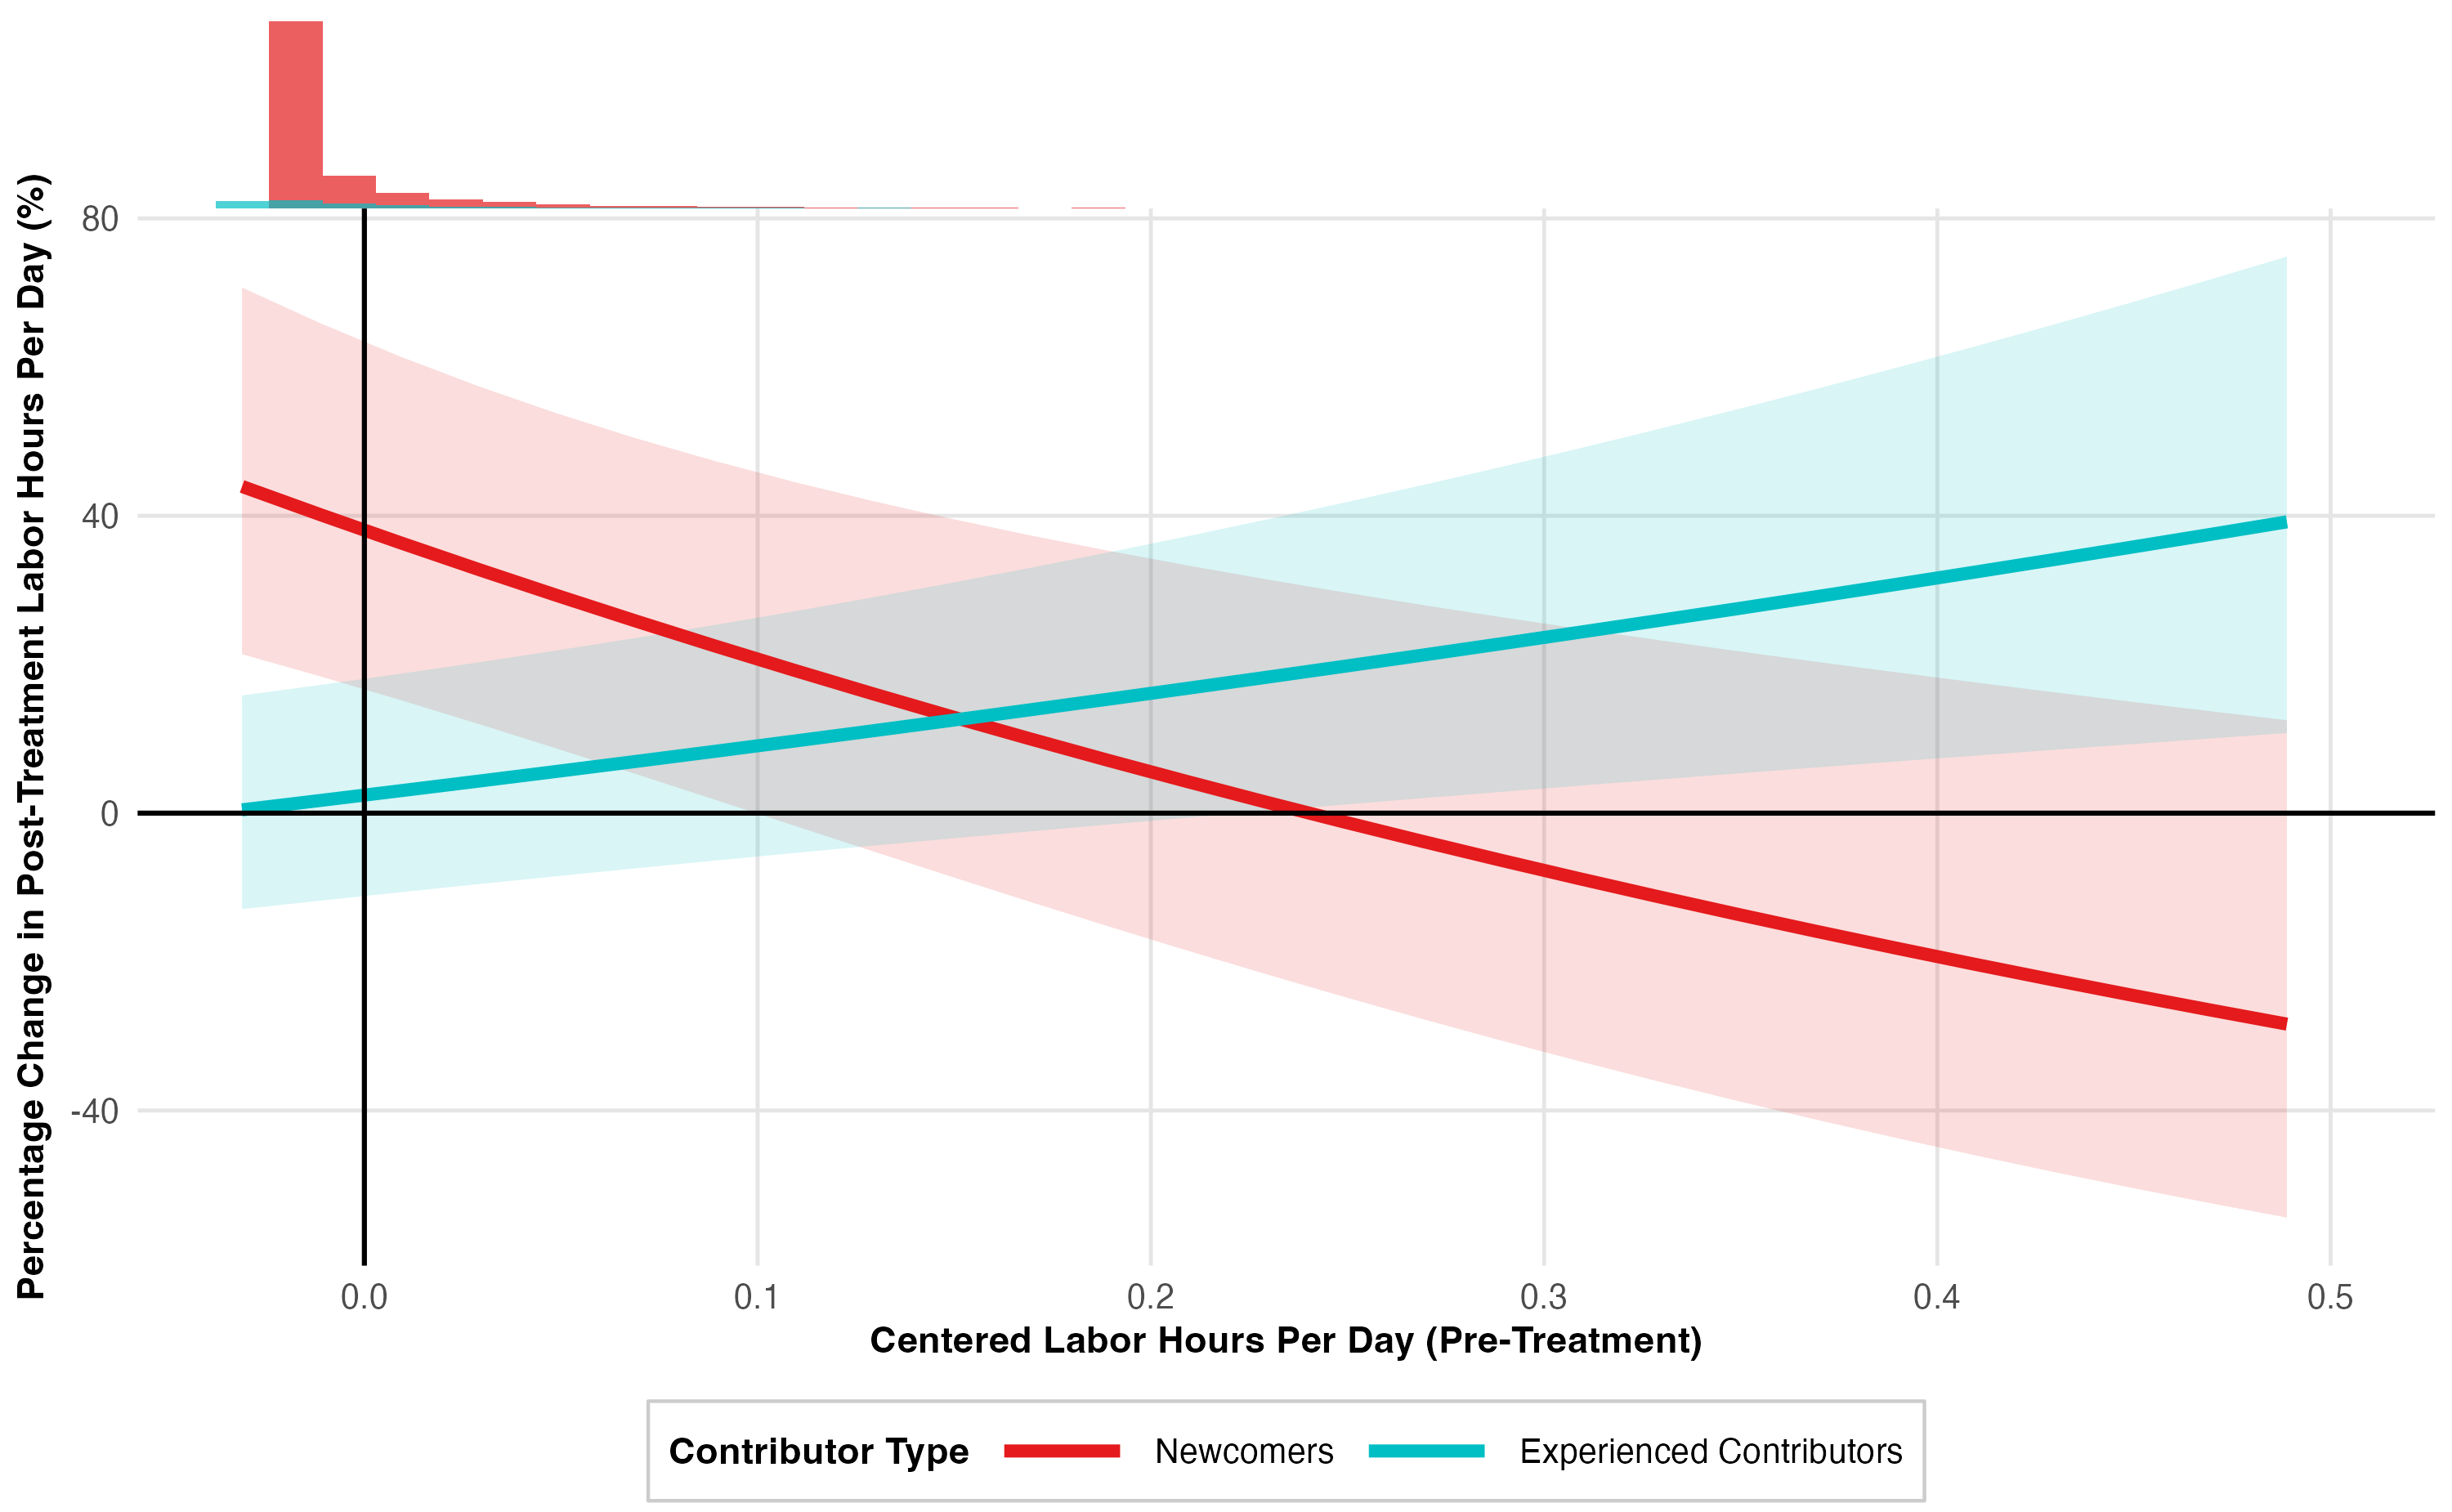
\includegraphics[width=0.9\linewidth]{figs/interaction_effect_marginal_histogram.png}
    \caption{The change in post-treatment labor hours per day in relation to centered pre-treatment labor hours per day for newcomers and experienced contributors (Table~\ref{table:full_labor_perday}). Histograms show the distribution of centered pre-treatment labor hours per day for each subgroup. The opposing slopes illustrate the contrasting interaction patterns: for newcomers, the gratitude effect diminishes with higher pre-treatment activity; for experienced contributors it is amplified.}
    \label{fig:labor.hours.interaction}
\end{figure}

\clearpage
\begin{figure}[h]
    \centering
    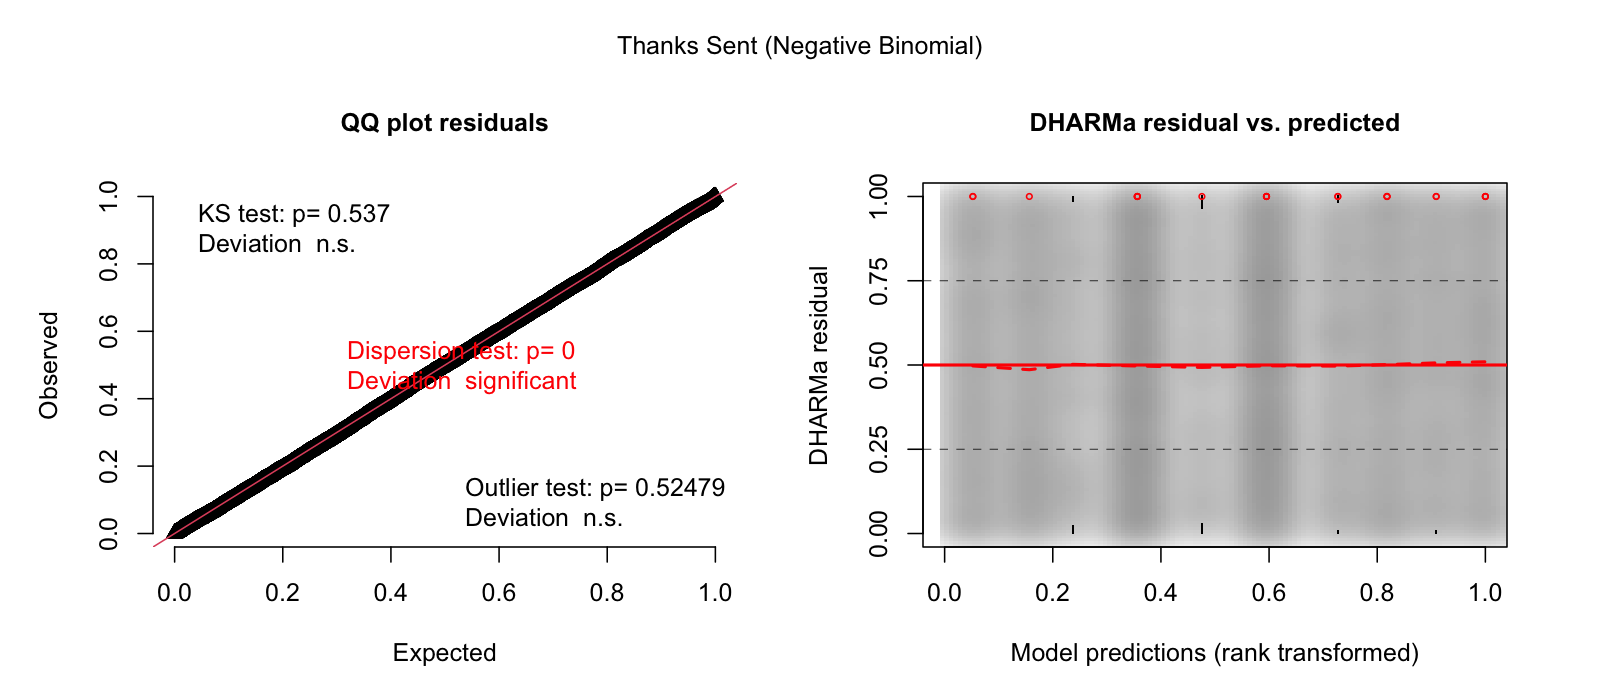
\includegraphics[width=0.95\linewidth]{figs/si_diagnostic_thanks_sent.png}
    \caption{DHARMa simulation-based residual diagnostics for the negative binomial model of thanks sent (all participants, $N = 15{,}274$). \textbf{Left:} QQ plot of randomized quantile residuals against the expected uniform distribution. The KS test ($p = 0.537$) indicates no significant deviation from uniformity, confirming adequate model specification. \textbf{Right:} Residuals versus model predictions (rank-transformed). The red lines show the empirical quantile trends; deviations from the horizontal reference lines (at 0.25, 0.50, and 0.75) would indicate misspecification. The dispersion test detected significant overdispersion ($p < 0.001$), which is common in large-sample count data but does not invalidate the negative binomial specification, as the negative binomial family explicitly models overdispersion relative to the Poisson.}
    \label{fig:negbin_dharma}
\end{figure}

\clearpage
\begin{figure}[h]
    \centering
    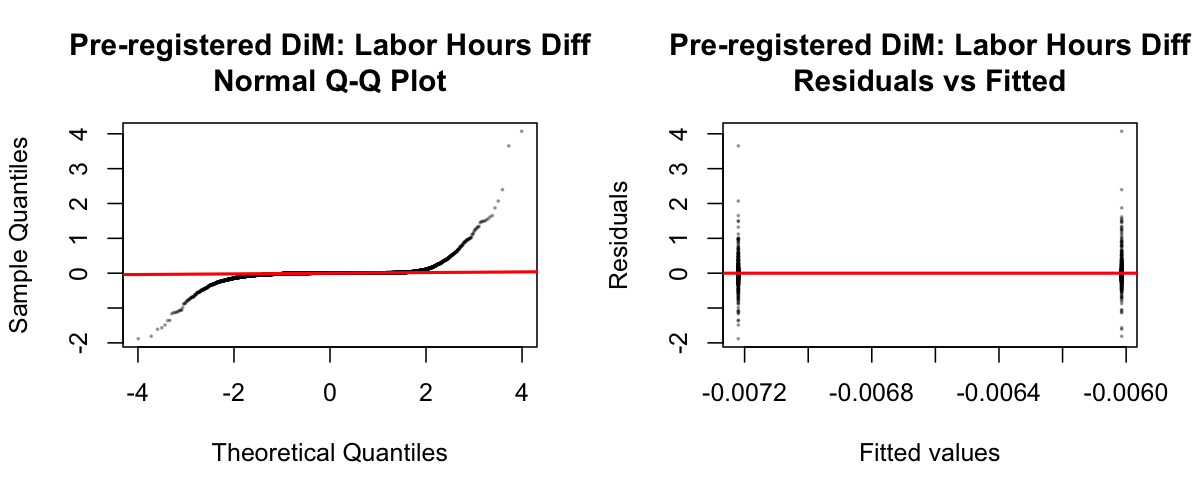
\includegraphics[width=0.95\linewidth]{figs/si_diagnostic_dim_labor_hours.png}
    \caption{Residual diagnostics for the pre-registered DiM model of labor hours (newcomers, $N = 9{,}984$). \textbf{Left:} Normal QQ plot showing severe departure from normality, with a heavy right tail reflecting the zero-inflated and highly right-skewed distribution of labor hours. \textbf{Right:} Residuals versus fitted values, revealing pronounced heteroscedasticity and non-constant variance. These violations of the linear model assumptions motivated the adoption of the Tweedie GLMM for analyzing labor hours outcomes.}
    \label{fig:dim_qq}
\end{figure}

\clearpage
\begin{figure}[h]
    \centering
    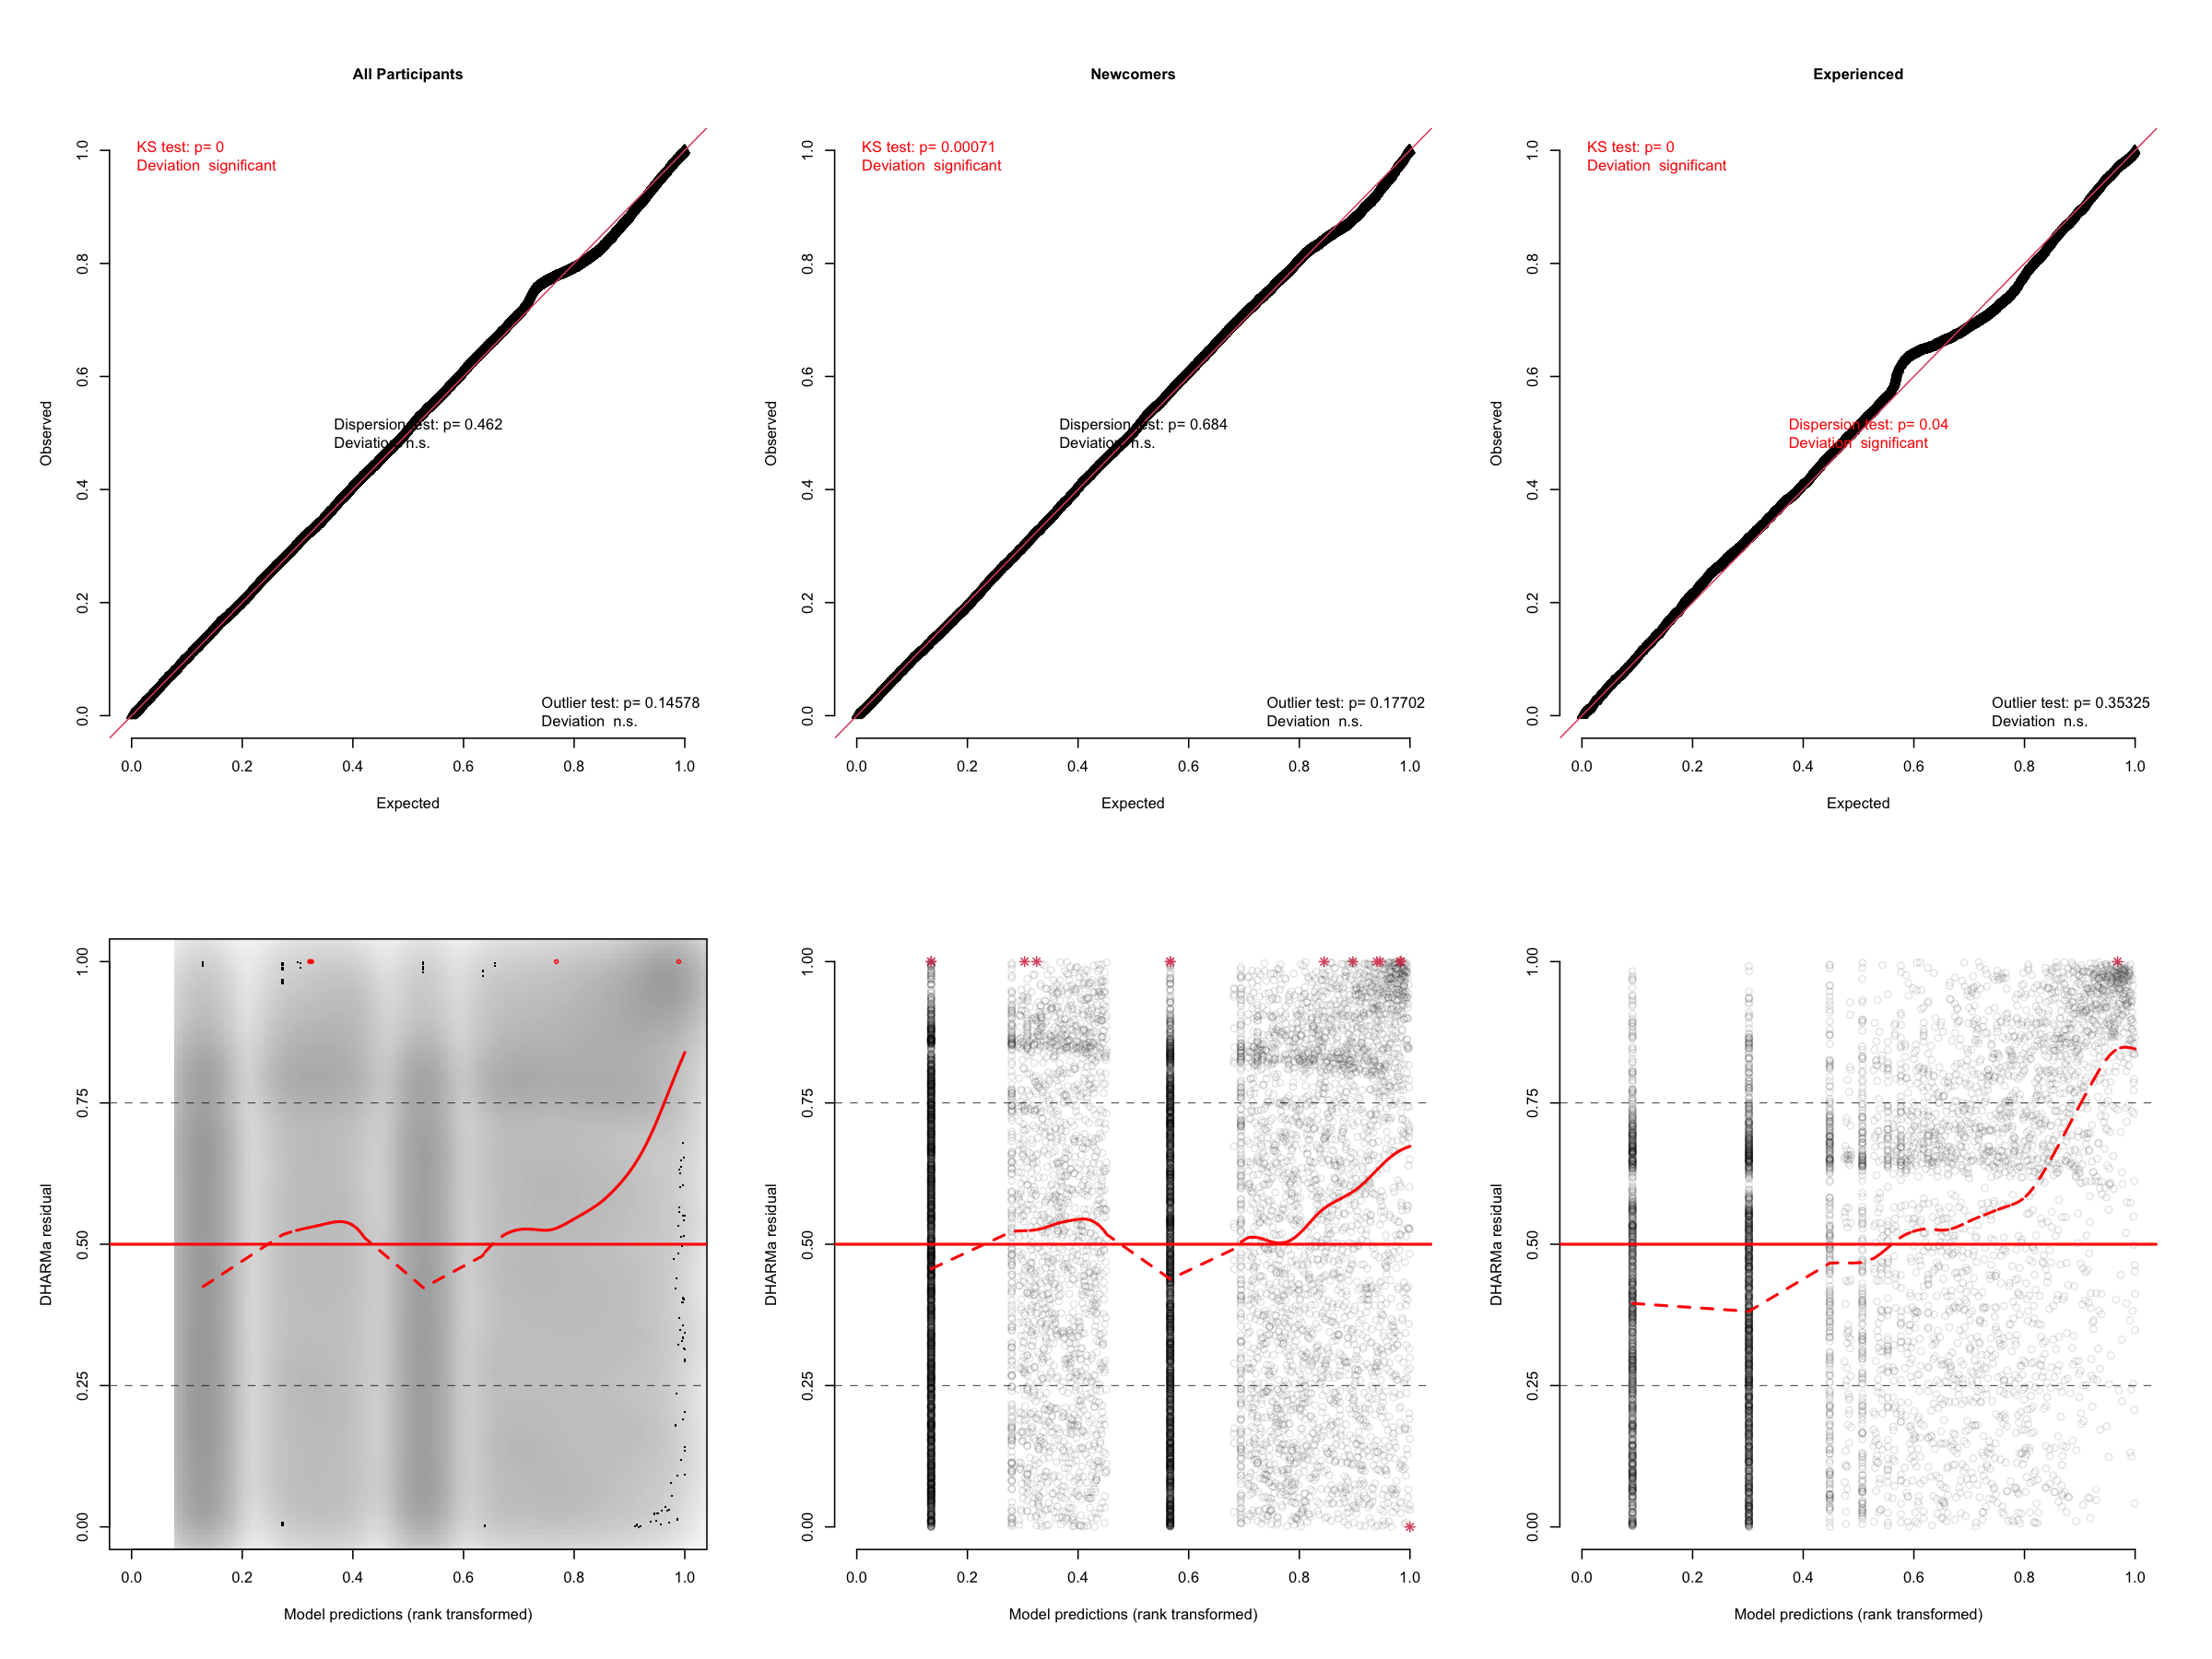
\includegraphics[width=0.95\linewidth]{figs/si_diagnostic_combined.png}
    \caption{DHARMa simulation-based residual diagnostics for the Tweedie GLMMs of post-treatment labor hours per day, shown separately for all participants ($N = 15{,}274$), newcomers ($N = 9{,}984$), and experienced contributors ($N = 5{,}290$). \textbf{Top row:} QQ plots of randomized quantile residuals. While the KS tests are significant due to the large sample sizes, the residuals closely follow the expected uniform distribution, with dispersion tests confirming adequate variance specification for all participants ($p = 0.462$) and newcomers ($p = 0.684$). The experienced subgroup shows mild dispersion ($p = 0.04$). \textbf{Bottom row:} Residuals versus model predictions (rank-transformed). Zero-inflation tests were non-significant for all three subgroups ($p > 0.10$), confirming that the Tweedie distribution adequately captures the excess zeros characteristic of labor hours data. These diagnostics support the use of Tweedie GLMMs over the pre-registered linear specification (Figure \ref{fig:dim_qq}).}
    \label{fig:tweedie_dharma}
\end{figure}

\clearpage
\begin{table*}[t]
\centering
\caption{Distribution of thanks by group, Wikipedia language edition, and participant experience level. Three columns correspond to three distinct types of thanks: \textit{First-Gen (Received)} = first-generation thanks sent by volunteers to treatment-group participants as part of the intervention ($N$ = total thanks in this category); \textit{Second-Gen (Treated)} = second-generation thanks subsequently sent by treated participants to other editors; \textit{Control (Sent)} = thanks sent by control-group participants who did not receive the intervention. Within each column, rows show the breakdown by language and experience level; percentages are column-wise (i.e., each column sums to 100\%).}
\label{table:thanks-distribution}
\begin{tabular}{lrrr}
\toprule
 & \textbf{First-Gen} & \textbf{Second-Gen} & \textbf{Control} \\
 & \textbf{(Received)} & \textbf{(Treated)} & \textbf{(Sent)} \\
 & (N = 2,806) & (N = 1,523) & (N = 1,066) \\
\midrule
\multicolumn{4}{l}{\textit{Experience level}} \\
\quad Experienced & 1,171 (41.7\%) & 1,119 (73.5\%) & 830 (77.9\%) \\
\quad Newcomer & 1,635 (58.3\%) & 404 (26.5\%) & 236 (22.1\%) \\
\addlinespace
\multicolumn{4}{l}{\textit{Language}} \\
\quad Arabic & 199 (7.1\%) & 43 (2.8\%) & 48 (4.5\%) \\
\quad German & 1,319 (47.0\%) & 285 (18.7\%) & 157 (14.7\%) \\
\quad Persian & 88 (3.1\%) & 432 (28.4\%) & 318 (29.8\%) \\
\quad Polish & 1,200 (42.8\%) & 763 (50.1\%) & 543 (50.9\%) \\
\addlinespace
\multicolumn{4}{l}{\textit{Language $\times$ Experience}} \\
\quad Arabic -- Newcomer & 199 (7.1\%) & 43 (2.8\%) & 48 (4.5\%) \\
\quad German -- Newcomer & 1,319 (47.0\%) & 285 (18.7\%) & 157 (14.7\%) \\
\quad Persian -- Experienced & 88 (3.1\%) & 432 (28.4\%) & 318 (29.8\%) \\
\quad Polish -- Newcomer & 117 (4.2\%) & 76 (5.0\%) & 31 (2.9\%) \\
\quad Polish -- Experienced & 1,083 (38.6\%) & 687 (45.1\%) & 512 (48.0\%) \\
\bottomrule
\end{tabular}
\end{table*}

\clearpage
\begin{figure}[h]
    \centering
    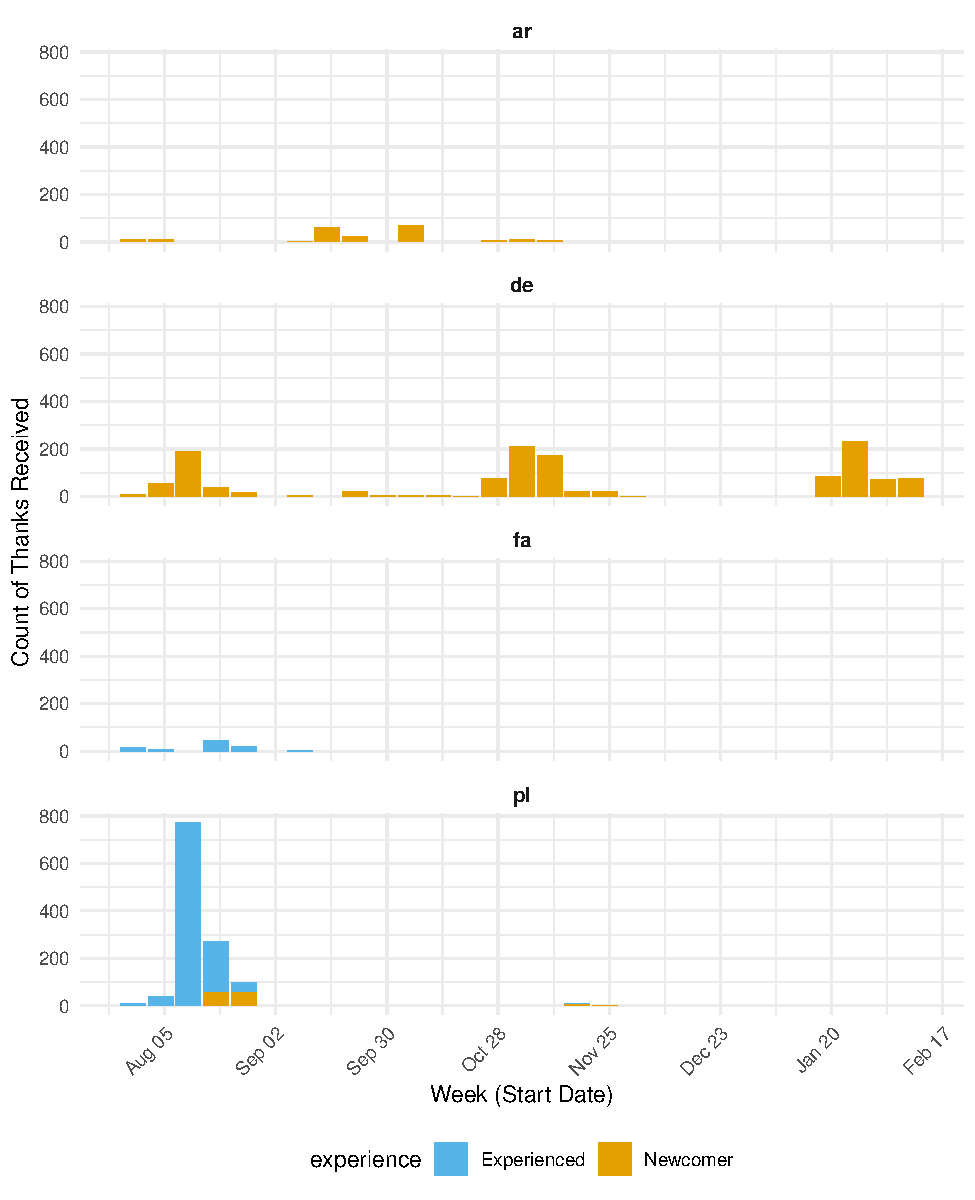
\includegraphics[width=0.9\linewidth]{figs/first.gen.thanks.pdf}
    \caption{The weekly count of first-generation thanks received by study participants, broken down by Wikipedia language edition (Arabic, German, Persian, Polish) and participant experience level (Newcomer vs. Experienced). First-generation thanks are those sent by the research team to treatment group participants as part of the experimental intervention. The stacked bars show how thanks were distributed over the study period, with each panel representing a different language community. The x-axis shows the start date of each week, with a 4-week break, and the y-axis shows the count of thanks received during that week.}
    \label{fig:first-gen-thanks}
\end{figure}

\clearpage
\begin{figure}[h]
    \centering
    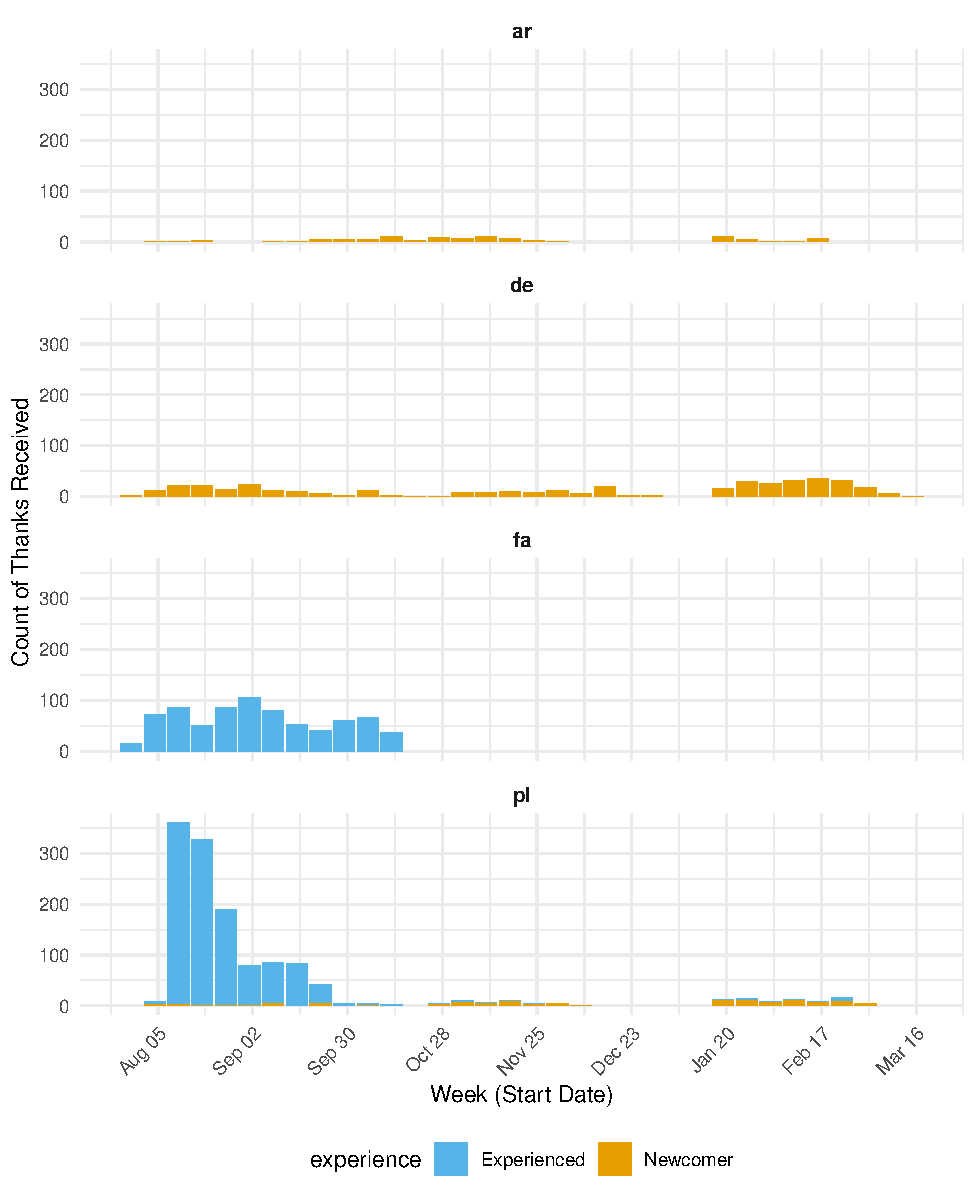
\includegraphics[width=0.9\linewidth]{figs/sec.gen.thanks.pdf}
    \caption{The weekly count of second-generation thanks sent by the treated participants who had previously received first-generation thanks, broken down by Wikipedia language edition (Arabic, German, Persian, Polish) and participant experience level (Newcomer vs. Experienced).  These are organic thanks sent by participants to other Wikipedia editors, representing the ``pay it forward'' behavior we hypothesized would result from receiving thanks. The stacked bars show how thanks were distributed over the study period, with each panel representing a different language community. The x-axis shows the start date of each week, with a 4-week break, and the y-axis shows the count of thanks received during that week. \textbf{Note:} Because participants were recruited in rolling waves, calendar dates reflect recruitment timing, not treatment timing. See Table~\ref{table:second-gen-sent} for onset-lag comparisons that account for this design feature.}
    \label{fig:second-gen-thanks}
\end{figure}

\clearpage
\begin{figure}[h]
    \centering
    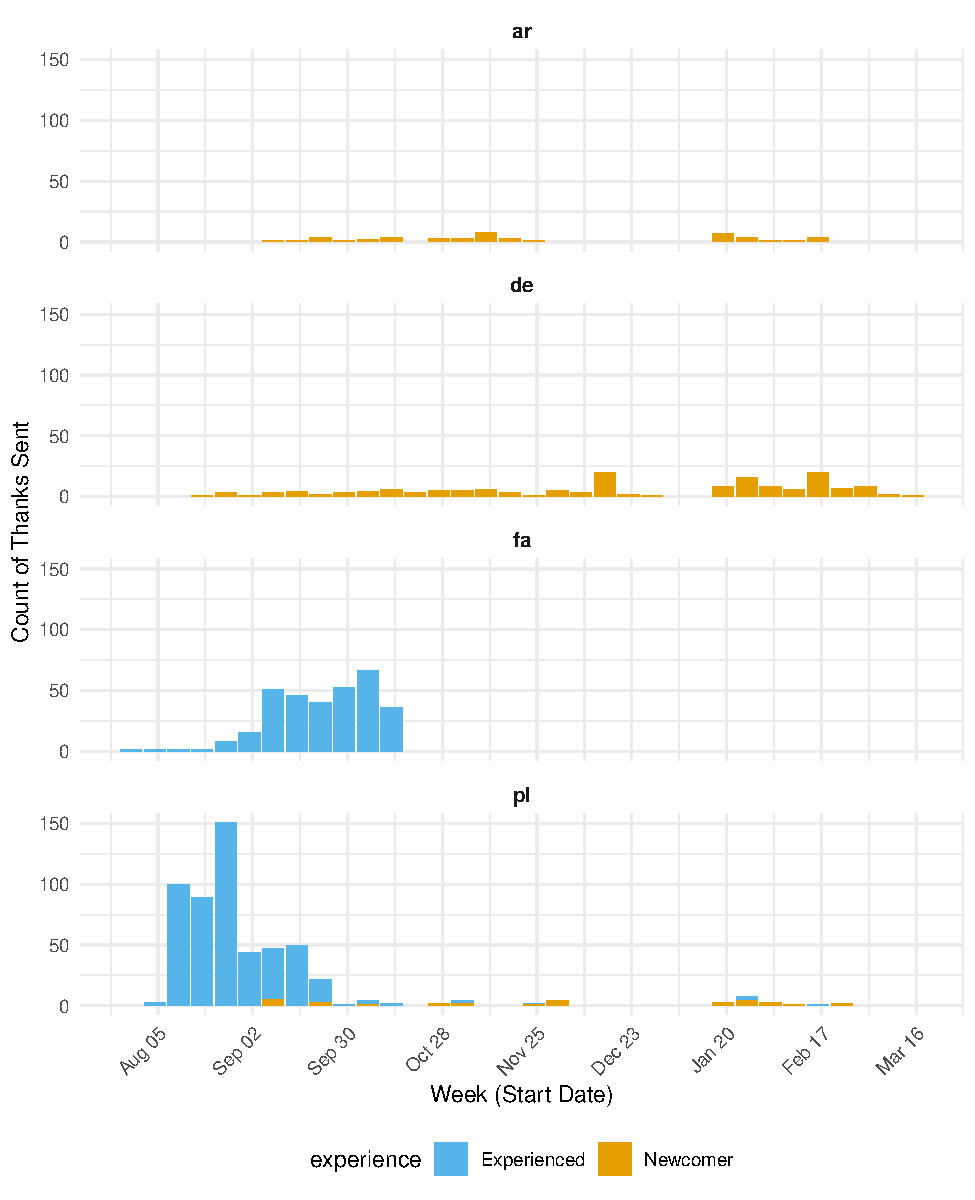
\includegraphics[width=0.9\linewidth]{figs/control.group.thanks.pdf}
    \caption{The weekly count of thanks sent by control group participants, broken down by Wikipedia language edition (Arabic, German, Persian, Polish) and participant experience level (Newcomer vs. Experienced). These participants did not receive first-generation thanks as part of the experimental intervention, so any thanks they sent represent baseline thanking behavior. The stacked bars show how thanks were distributed over the study period, with each panel representing a different language community. The x-axis shows the start date of each week, with a 4-week break, and the y-axis shows the count of thanks sent during that week. \textbf{Note:} Because participants were recruited in rolling waves, calendar dates reflect recruitment timing, not treatment timing. See Table~\ref{table:second-gen-sent} for onset-lag comparisons that account for this design feature.}
    \label{fig:control-thanks}
\end{figure}

\clearpage
\begin{figure}[h]
    \centering
    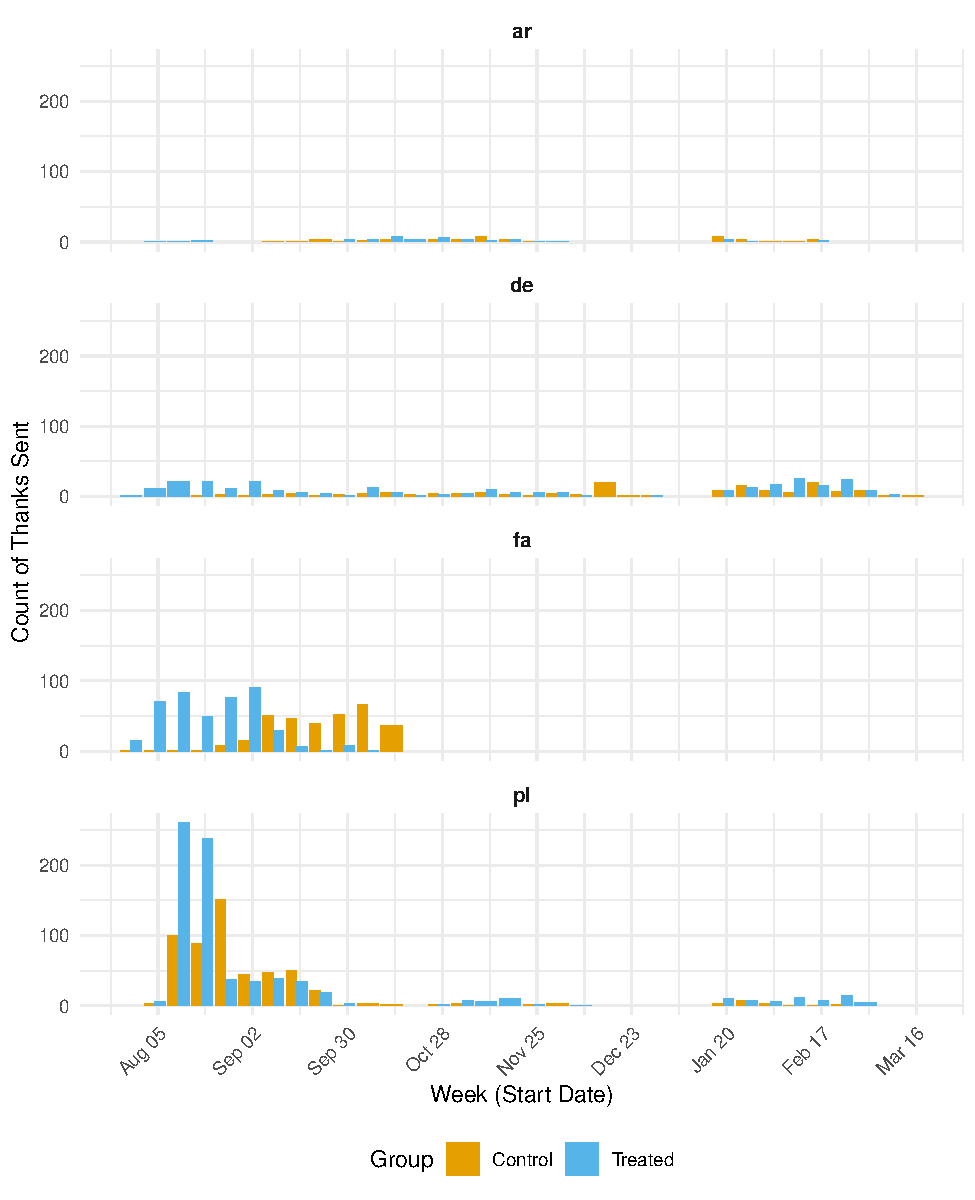
\includegraphics[width=0.9\linewidth]{figs/treated.vs.control.thanks.pdf}
    \caption{A comparison of the weekly count of thanks sent by treated and control group participants, broken down by Wikipedia language edition (Arabic, German, Persian, Polish). Treated participants received first-generation thanks as part of the experimental intervention, while control participants did not. The side-by-side bars allow direct comparison of thanking behavior between the two groups over the study period. Each panel represents a different language community. The x-axis shows the start date of each week, with a 4-week break, and the y-axis shows the count of thanks sent during that week. \textbf{Note:} Because participants were recruited in rolling waves, calendar dates reflect recruitment timing, not treatment timing. Apparent temporal differences between groups in this figure should not be interpreted as onset-lag effects; see Table~\ref{table:second-gen-sent} for onset-lag comparisons that account for this design feature.}
    \label{fig:treated-vs-control-thanks}
\end{figure}

\clearpage
\begin{table}[ht]
\centering
\small
\caption{Second-generation thanks \emph{sent} by treated and control group participants, by Wikipedia language edition. Because participants were recruited in rolling waves, we report the \emph{onset lag} as the median number of days from the first-generation thanks date to the date each participant sent their \emph{first} second-generation thanks, rather than absolute calendar dates. Each unique sender contributes one observation. The baseline date is when the volunteer application sent first-generation thanks to the treated participant in each matched pair; both treated and control participants in the same pair use this same date, making the comparison within-pair and directly comparable. Onset lags were similar across groups (11--16~days), indicating that the treatment effect operated through increased volume and intensity of thanking rather than earlier initiation. Arabic is the only language where control participants sent more total thanks than treated participants (48 vs.\ 43) and had more unique senders (19 vs.\ 17), likely reflecting its small and dense editing community. In Polish Wikipedia, treated and control participants had nearly equal numbers of unique senders (109 vs.\ 107), yet treated senders sent 37\% more thanks per sender (7.0 vs.\ 5.1), illustrating that the treatment effect operated through \emph{intensity} of thanking rather than participation rate.}
\label{table:second-gen-sent}
\begin{tabular}{ll rrr rr}
\toprule
\textbf{Language} & \textbf{Group} & \textbf{Thanks} & \textbf{Unique Senders} & \textbf{Thanks/Sender} & \textbf{Onset Lag (d)} & \textbf{Interquartile Range (d)} \\
\midrule
Arabic & Treated &  43 & 17 & 2.5 & 15 & [4, 25] \\
       & Control &  48 & 19 & 2.5 & 16 & [9, 26] \\
\addlinespace
German & Treated & 266 & 78 & 3.4 & 15 & [6, 23] \\
       & Control & 139 & 53 & 2.6 & 15 & [5, 30] \\
\addlinespace
Persian & Treated & 432 & 62 & 7.0 & 14 & [5, 26] \\
        & Control & 318 & 43 & 7.4 & 11 & [3, 25] \\
\addlinespace
Polish & Treated & 763 & 109 & 7.0 & 15 & [5, 26] \\
       & Control & 543 & 107 & 5.1 & 12 & [5, 21] \\
\addlinespace
\textbf{Total} & \textbf{Treated} & \textbf{1{,}504} & \textbf{266} & \textbf{5.7} & \textbf{15} & \textbf{[5, 25]} \\
 & \textbf{Control} & \textbf{1{,}048} & \textbf{222} & \textbf{4.7} & \textbf{13} & \textbf{[4, 25]} \\
\bottomrule
\end{tabular}
\end{table}

\clearpage
\begin{table}[ht]
\centering
\small
\caption{Cross-tabulation of second-generation thanks \emph{received} by Wikipedia language edition, sender group, and recipient status. Each language block contains three rows: thanks sent by treated participants, thanks sent by control participants, and an italic \emph{All} row totalling both. Columns classify each thank by the recipient's study enrollment: \textit{Treated Recip.}\ = study-enrolled treated participant; \textit{Control Recip.}\ = study-enrolled control participant; \textit{Non-participant} = Wikipedia editor outside the study; \textit{Total} = row sum. The \textit{Unique Ctrl.\ Recip.}$^\dagger$ column is the key spillover measure: it counts the \emph{distinct} control participants who received a second-generation thank from a treated sender \emph{verified} to have actually received a first-generation thank (i.e., a non-null volunteer sender is recorded in the data). Treated participants who were assigned to treatment but never received the thank are excluded from this count because the volunteer skipped them, the notification expired unseen, or the account was deleted. This column is only populated for Treated-sender rows; ``--'' in Control-sender rows indicates the column is not applicable, and blank cells in \emph{All} rows indicate the aggregate is not meaningful. In Persian Wikipedia, the 74 thanks received by control participants split roughly evenly between treated senders (32) and control senders (42); in Polish Wikipedia the split was similarly even (63 vs.\ 67), indicating that second-generation thanks circulated through the small active editing communities regardless of treatment assignment. In total, 49 unique control participants (0.6\% of all controls) were reached via the verified treatment-spillover pathway; the implications of this spillover for the ITT estimate are assessed in the Spillover Sensitivity Analysis section.}
\label{table:second-gen-received}
\begin{tabular}{ll rrrrr}
\toprule
\textbf{Language} & \textbf{Sender} & \textbf{Treated Recip.} & \textbf{Control Recip.} & \textbf{Unique Ctrl. Recip.}$^\dagger$ & \textbf{Non-participant} & \textbf{Total} \\
\midrule
Arabic & Treated &   3 &   3 &  3 &  37 &  43 \\
       & Control &   8 &   3 & -- &  37 &  48 \\
       & \textit{All} & \textit{11} & \textit{6} & & \textit{74} & \textit{91} \\
\addlinespace
German & Treated &   5 &   6 &  5 & 255 & 266 \\
       & Control &   3 &   1 & -- & 135 & 139 \\
       & \textit{All} & \textit{8} & \textit{7} & & \textit{390} & \textit{405} \\
\addlinespace
Persian & Treated &  72 &  32 &  4 & 328 & 432 \\
        & Control &  52 &  42 & -- & 224 & 318 \\
        & \textit{All} & \textit{124} & \textit{74} & & \textit{552} & \textit{750} \\
\addlinespace
Polish & Treated & 475 &  63 & 37 & 225 & 763 \\
       & Control & 273 &  67 & -- & 203 & 543 \\
       & \textit{All} & \textit{748} & \textit{130} & & \textit{428} & \textit{1{,}306} \\
\addlinespace
\textbf{Total} & \textbf{Treated} & \textbf{555} & \textbf{104} & \textbf{49} & \textbf{845} & \textbf{1{,}504} \\
 & \textbf{Control} & \textbf{336} & \textbf{113} & \textbf{--} & \textbf{599} & \textbf{1{,}048} \\
 & \textbf{\textit{All}} & \textbf{\textit{891}} & \textbf{\textit{217}} & & \textbf{\textit{1{,}444}} & \textbf{\textit{2{,}552}} \\
\bottomrule
\end{tabular}
\end{table}

\clearpage
\begin{table}[ht]
\centering
\small
\caption{Second-generation thanks and community context, by Wikipedia language edition. ``Active editors'' is the average monthly count of editors with at least one edit during the study period (August~2019 -- February~2020). ``Study participants'' is the total number of editors enrolled in the experiment (recruited from cumulative editing activity, so this count may exceed the monthly active editor count). ``Unique senders'' and ``unique recipients'' count distinct individuals who sent or received at least one second-generation thank. ``Non-participant recipients'' counts unique recipients not enrolled in the study. ``Recipients / sender'' is the mean number of distinct recipients per sender. ``Thanks / 1{,}000 active'' standardizes total second-generation thanks by community size.}
\label{table:second-gen-community}
\begin{tabular}{l rr rr r r r}
\toprule
\textbf{Language} & \textbf{Active Editors} & \textbf{Study Partic.} & \textbf{Unique Senders} & \textbf{Unique Recip.} & \textbf{Non-Part. Recip.} & \textbf{Recip./Sender} & \textbf{Thanks/1{,}000 Active} \\
\midrule
Arabic  &    959 & 3{,}072 &  36 &   49 &  38 & 1.4 &   95 \\
German  & 6{,}348 & 5{,}416 & 131 &  247 & 237 & 1.9 &   64 \\
Persian & 1{,}317 & 2{,}413 & 105 &  195 & 117 & 1.9 &  570 \\
Polish  & 1{,}462 & 4{,}528 & 216 &  906 & 151 & 4.2 &  893 \\
\bottomrule
\end{tabular}
\end{table}

\clearpage
\begin{figure}[h]
    \centering
    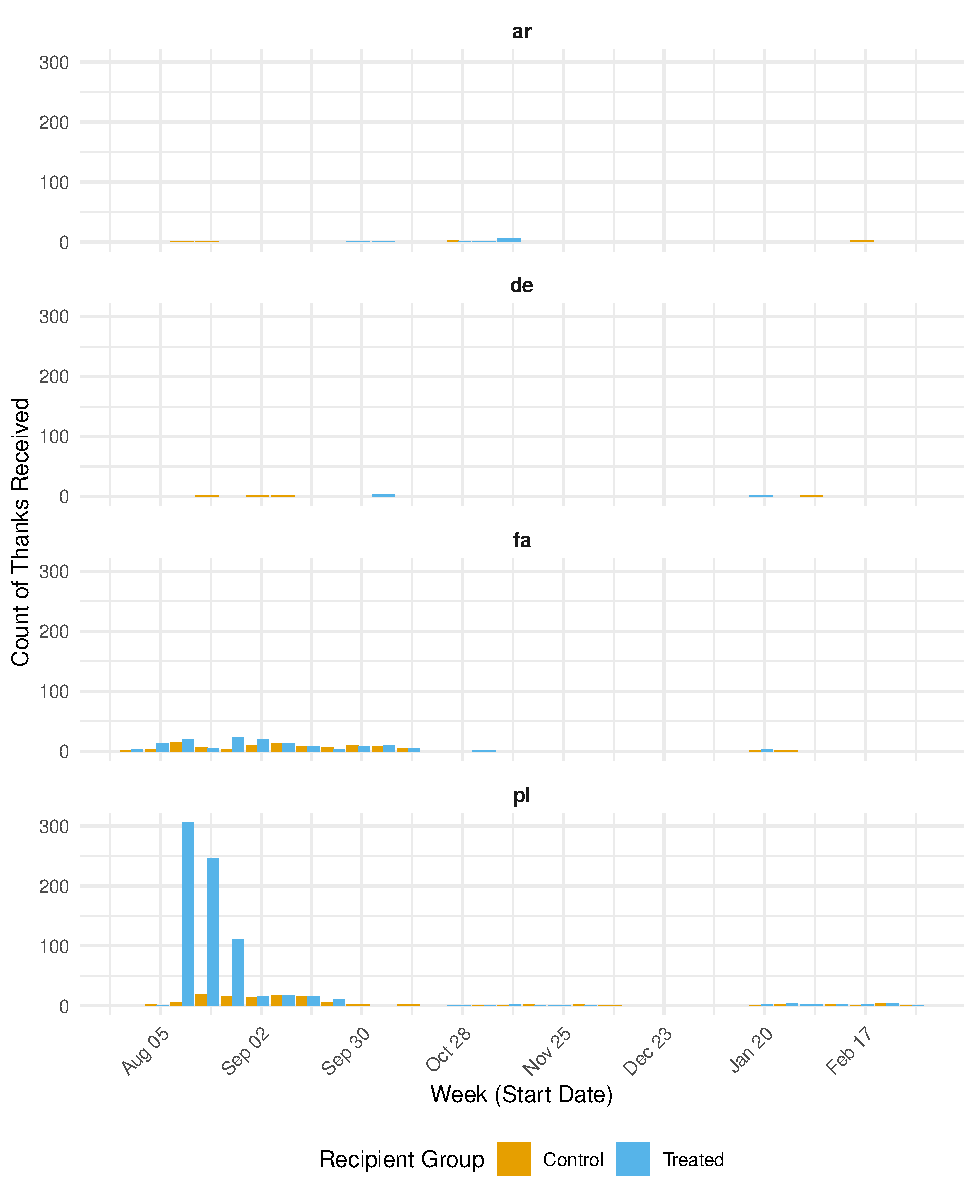
\includegraphics[width=0.9\linewidth]{figs/second.gen.received.by.group.pdf}
    \caption{The weekly count of second-generation thanks \emph{received} by study participants, broken down by recipient group (Treated vs.\ Control) and Wikipedia language edition (Arabic, German, Persian, Polish). Each panel shows one language community with free y-axis scales to accommodate the different volumes. In Persian Wikipedia, control participants received 74 second-generation thanks compared to 124 for treated participants, and in Polish Wikipedia 130 compared to 748, despite control participants not being targeted by the intervention. This pattern is consistent with the limited recipient pool in smaller communities causing thanks to circulate back to control group members.}
    \label{fig:received-by-group}
\end{figure}

\clearpage
\begin{figure}[h]
    \centering
    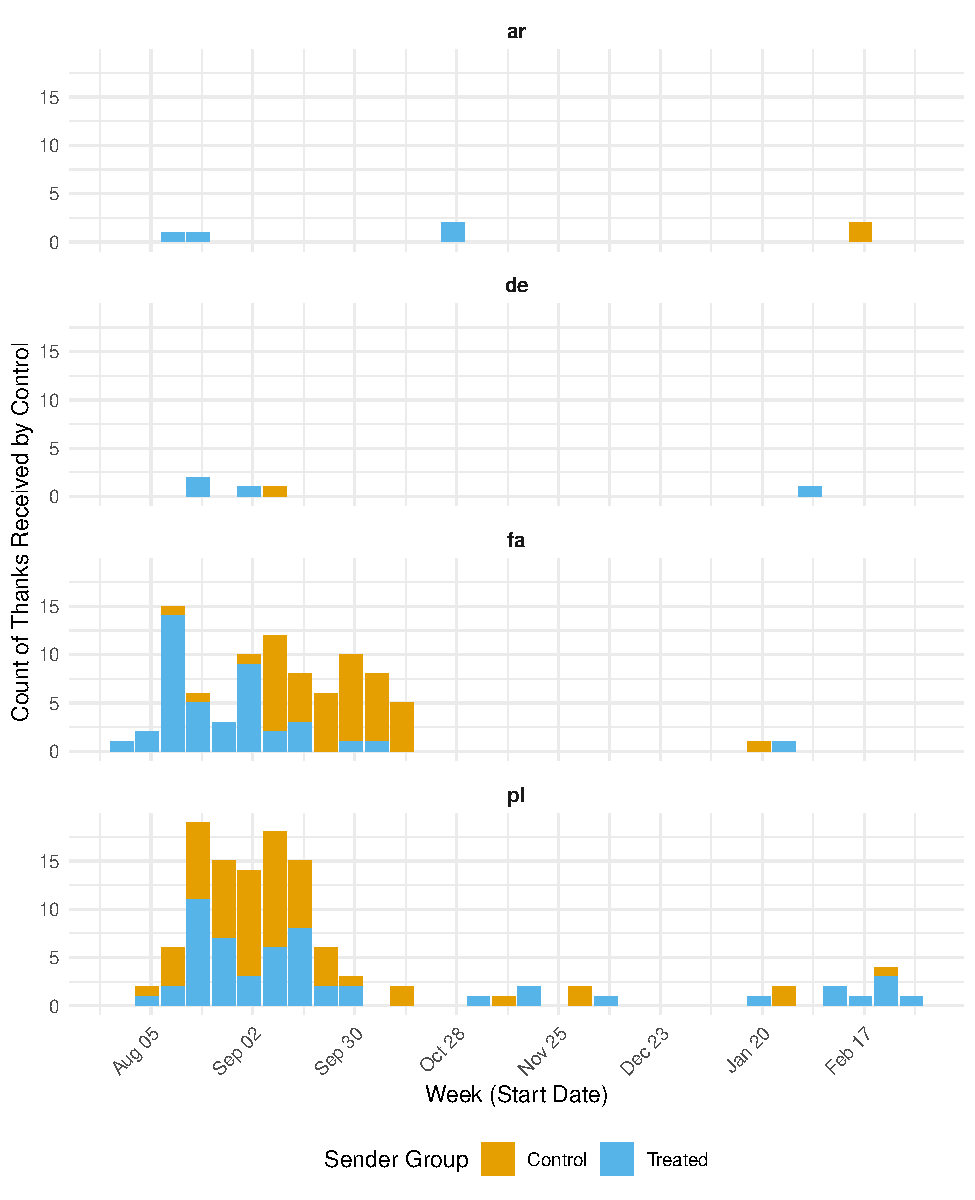
\includegraphics[width=0.9\linewidth]{figs/control.received.thanks.by.sender.pdf}
    \caption{The weekly count of second-generation thanks \emph{received} by control group participants, broken down by who sent the thanks (Treated sender vs.\ Control sender) and Wikipedia language edition (Arabic, German, Persian, Polish). In Persian Wikipedia, thanks received by control participants came roughly equally from treated senders (32 total) and control senders (42 total). In Polish Wikipedia, 67 came from control senders and 63 from treated senders. This near-parity suggests that the ``pay it forward'' thanking behavior occurred across the community irrespective of the original treatment assignment, with the small active editing pool causing thanks to circulate back to control participants.}
    \label{fig:control-received-by-sender}
\end{figure}


\clearpage
\begin{table}[ht]
\centering
\small
\caption{Second-generation thanks sending rates among control-group participants, comparing those who received at least one second-generation thank from a verified treated sender (``Exposed,'' $n = 49$) with those who did not (``Unexposed,'' $n = 7{,}662$). A treated sender is ``verified'' if a non-null volunteer sender is recorded in the data, confirming they actually received first-generation thanks. ``Sent thanks'' is the count who sent at least one second-generation thank; ``Sending rate'' is that count divided by $N$. The ``All controls'' row shows the pooled rate across both groups. The 9$\times$ rate difference (24.5\% vs.\ 2.7\%) is consistent with a spillover pathway but should be interpreted cautiously: exposed controls are likely more active editors who would send thanks regardless of the exposure, so this comparison is correlational rather than causal.}
\label{table:exposure-response}
\begin{tabular}{l rrr}
\toprule
\textbf{Control group} & \textbf{$N$} & \textbf{Sent thanks} & \textbf{Sending rate} \\
\midrule
Unexposed & 7{,}662 & 210 & 2.7\% \\
Exposed   &     49 &  12 & 24.5\% \\
\midrule
All controls & 7{,}711 & 222 & 2.9\% \\
\bottomrule
\end{tabular}
\end{table}

\clearpage
\begin{table}[ht]
\centering
\small
\caption{Sensitivity analysis comparing the standard and spill-over adjusted RD for second-generation thanks sending. Each row reports the proportion of participants who sent at least one second-generation thank (\textit{Treated rate} and \textit{Control rate}), and the resulting risk difference in percentage points (\textit{RD (pp)} = treated rate $-$ control rate). The \textit{Standard ITT} row uses all 7{,}711 control participants. The \textit{Spill-over adjusted ITT} row excludes the 49 control participants who received a second-generation thank from a verified treated sender (Table~\ref{table:exposure-response}), thereby removing those most likely to have been indirectly affected by the treatment; the control group shrinks to 7{,}662. The treated rate is identical in both rows because no treated participants are excluded. The spill-over adjusted RD of 0.71 percentage points is 24\% larger than the standard RD of 0.57 percentage points, indicating that indirect exposure modestly inflated the control group's outcome and that the standard ITT is a conservative lower bound on the direct effect.}
\label{table:purified-itt}
\begin{tabular}{l r r r}
\toprule
\textbf{Estimate} & \textbf{Treated rate} & \textbf{Control rate ($N$)} & \textbf{RD (pp)} \\
\midrule
Standard ITT & 3.45\% & 2.88\% ($N = 7{,}711$) & $+$0.57 \\
Spill-over adjusted ITT & 3.45\% & 2.74\% ($N = 7{,}662$) & $+$0.71 \\
\bottomrule
\end{tabular}
\end{table}

\FloatBarrier

\bibliography{references}

\end{document}
